\chapter{Finite element method: implementation}

\section{Introduction}
\begin{equation*}
  \hat A_{h,ij} = a(\phi_j,\phi_i)
\end{equation*}

\begin{equation*}
  \hat A^K_{\alpha\beta} = \int_K \pp{\phi^K_\beta}{x_i} a_{ij} \pp{\phi^K_\alpha}{x_j} dx
\end{equation*}

We need three key ingredients
\begin{itemize}
\item[1.] a means to evaluate basis function values and gradients at any points in a reference element $\tilde K$.
\item[2.] a means to transform the integral over the element $K$ to an integral over the reference element $\tilde K$.
\item[3.] a means to approximate the integral over the reference element $\tilde K$ using a quadrature rule.
\end{itemize}

As we have seen in Lecture~\ref{ch:pos1d}, the computation of a finite element solution requires a few common tasks on the functions in $\calV_h$, such as the evaluation of the function values, the valuation of the gradient values, and the integration of the functions.  Our approach to construct the piecewise polynomial space is to first define a polynomial space on a \emph{reference element} (or a \emph{canonical element}) and then to map the polynomial functions to the actual elements that comprise the triangulation.  


\section{Linear Lagrange finite element on a triangle}
\label{sec:fe_lin_tri}
We first introduce the \emph{reference triangle} $\tilde K$.  (Note that all quantities associated with the reference space bear tilde ($\tilde \cdot$).) While the definition of a reference triangle is not universal, our reference triangle, as shown in Figure~\ref{fig:fe_ref_tri}, is a right triangle delineated by three vertices
\begin{equation*}
  \tilde v_1 \equiv (0,0), \quad \tilde v_2 \equiv (1,0), \quad \text{and} \quad \tilde v_3 \equiv (0,1).
\end{equation*}
The vertices are ordered in the counter-clockwise manner, starting with the first vertex at the origin. We also denote the three edges of the triangles by
\begin{equation*}
  \tilde e_1 \equiv ( \tilde v_2, \tilde v_3), \quad  \tilde e_2 \equiv ( \tilde v_3, \tilde v_1), \quad \text{and} \quad  \tilde e_3 \equiv ( \tilde v_1, \tilde v_2).
\end{equation*}
We choose the convention that the edge number is the same as the vertex number of the vertex on the other side of the triangle. Each edge is oriented such that the collection of the three edges defines the triangle in the counter-clockwise orientation.  

\begin{figure}
  \centering
  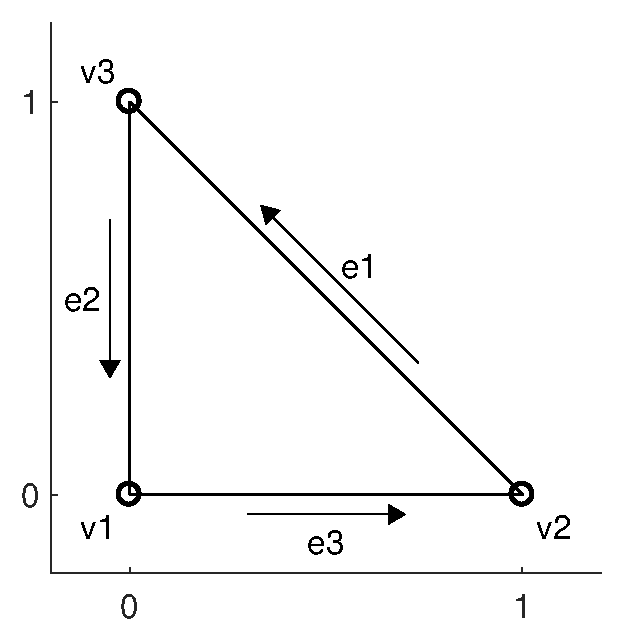
\includegraphics[width=0.3\textwidth]{ref_tri}
  \caption{Reference triangle $\tilde K$.}
  \label{fig:fe_ref_tri}
\end{figure}

Having introduced the reference triangle, we now introduce the linear Lagrange finite element on the reference triangle. A linear function in $\PP^1(\tilde K)$ takes on the form $a_1 + a_2 \tilde x_1 + a_3 \tilde x_2$ and has three degrees of freedom; we hence need to identify a linear independent set of three linear functions.  In our case, we wish to identify a set of three linear \emph{Lagrange basis functions} for the space.  To this end, we choose for our Lagrange interpolation nodes the three vertices of the triangle
\begin{equation*}
  \tilde z_1 = (0,0), \quad \tilde z_2 = (1,0), \quad \text{and} \quad \tilde z_3 = (0,1),
\end{equation*}
as shown in Figure~\ref{fig:fe_ref_tri_p1}. Our goal is to find the Lagrange basis 
\begin{equation*}
  \{ \tilde \phi_1, \tilde \phi_2, \tilde \phi_3 \}
\end{equation*}
that lie in the $\PP^1(\tilde K)$ space and satisfy the interpolation condition
\begin{equation}
  \tilde \phi_i(\tilde z_j) = \delta_{ij} \quad i,j = 1,\dots,3.
   \label{eq:fe_interp_tri}
\end{equation}
Here, $\delta_{ij}$ denotes the \emph{Kronecker delta} such that $\delta_{ij} = 1$ for $i = j$ and $\delta_{ij} = 0$ for $i \neq j$.

\begin{figure}
  \centering
  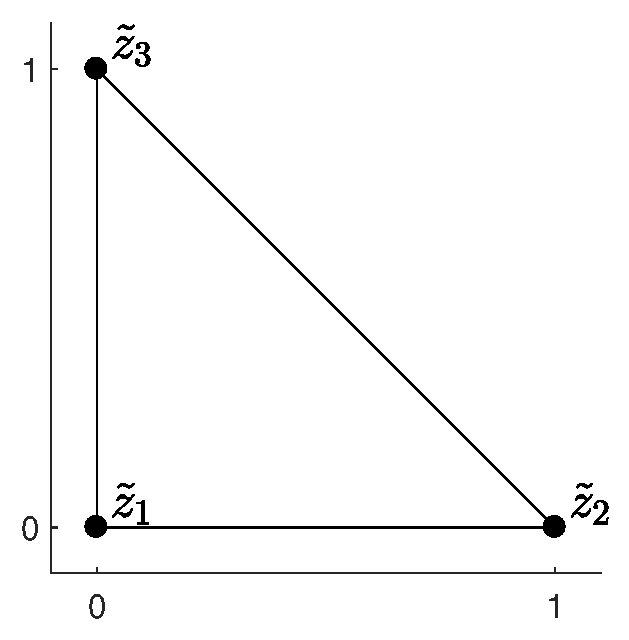
\includegraphics[width=0.3\textwidth]{ref_tri_p1}
  \caption{Linear Lagrange finite element on the reference triangle.}
  \label{fig:fe_ref_tri_p1}
\end{figure}

    While we may identify the Lagrange basis functions for $\PP^1(\tilde K)$ by inspection, we here follow a more systematic procedure that apply to more complex domains and higher-order polynomials.  To this end, we first note that any linear function can be expressed as a linear combination of a monomial basis
\begin{equation*}
  \{ 1, \tilde x_1, \tilde x_2\}.
\end{equation*}
Since linear Lagrange basis functions are also linear functions, we can express the basis functions in terms of the monomial basis:
\begin{equation}
  \tilde \phi_j(\tilde x) = c^{(j)}_1 + c^{(j)}_2 \tilde x_1 + c_3^{(j)} \tilde x_2 \quad j = 1, 2, 3.
  \label{eq:fe_lin_tri_rep}
\end{equation}
We now apply the interpolation condition~\eqref{eq:fe_interp_tri} to find the coefficients.  For instance, $\tilde \phi_1$ must satisfy
\begin{equation*}
  \bmat{ccc}
  1 & \tilde z_{1,1} & \tilde z_{1,2} \\
  1 & \tilde z_{2,1} & \tilde z_{2,2} \\
  1 & \tilde z_{3,1} & \tilde z_{3,2} \\
  \emat
  \bmat{ccc}
  c_1^{(1)} \\ c_2^{(1)} \\ c_3^{(1)}
  \emat
  =
  \bmat{ccc}
  1 \\ 0 \\ 0,
  \emat
\end{equation*}
where $\tilde z_{i,j}$ is the $j$-th coordinate of the $i$-th interpolation node. We can also pose a single matrix equation for the monomial coefficients of all three shape functions: 
\begin{equation*}
  \underbrace{
   \bmat{ccc}
  1 & \tilde z_{1,1} & \tilde z_{1,2} \\
  1 & \tilde z_{2,1} & \tilde z_{2,2} \\
  1 & \tilde z_{3,1} & \tilde z_{3,2} \\
  \emat }_{\equiv V}
  \underbrace{ 
  \bmat{ccc}
  c_1^{(1)} & c_1^{(2)} & c_1^{(3)} \\
  c_2^{(1)} & c_2^{(2)} & c_2^{(3)} \\
  c_3^{(1)} & c_3^{(2)} & c_3^{(3)} \\
  \emat
  }_{\equiv C}
  =
  \bmat{ccc}
  1 & 0 & 0 \\
  0 & 1 & 0 \\
  0 & 0 & 1
  \emat.
\end{equation*}
The matrix $V$ in the left hand side is the \emph{Vandermonde matrix} associated with our monomial basis evaluated at the Lagrange interpolation points $\{\tilde z_1,\tilde z_2, \tilde z_3\}$.  The matrix $V$ is non-singular as long as the interpolation points are not collinear, which is equivalent to the condition that the triangle have a finite area; the condition is obviously satisfied for our reference triangle $\tilde K$. Hence the unique coefficients are given by $C \equiv V^{-1}$.  For completeness, we provide the explicit expression for the coefficients 
\begin{equation*}
  C = \bmat{ccc}
  1 & 0 & 0\\
  -1 & 1 & 0 \\
  -1 & 0 & 1
  \emat;
\end{equation*}
the associated basis functions are
\begin{align}
  \tilde \phi_1(\tilde x) &= 1 - \tilde x_1 - \tilde x_2 \notag \\
  \tilde \phi_2(\tilde x) &= \tilde x_1 \label{eq:fe_lin_tri_expl} \\
  \tilde \phi_3(\tilde x) &= \tilde x_2. \notag
\end{align}
Figure~\ref{fig:fe_shape_tri_p1} visualizes the three basis functions.

\begin{figure}
  \centering
  \subfigure[$\tilde \phi_1$]{
    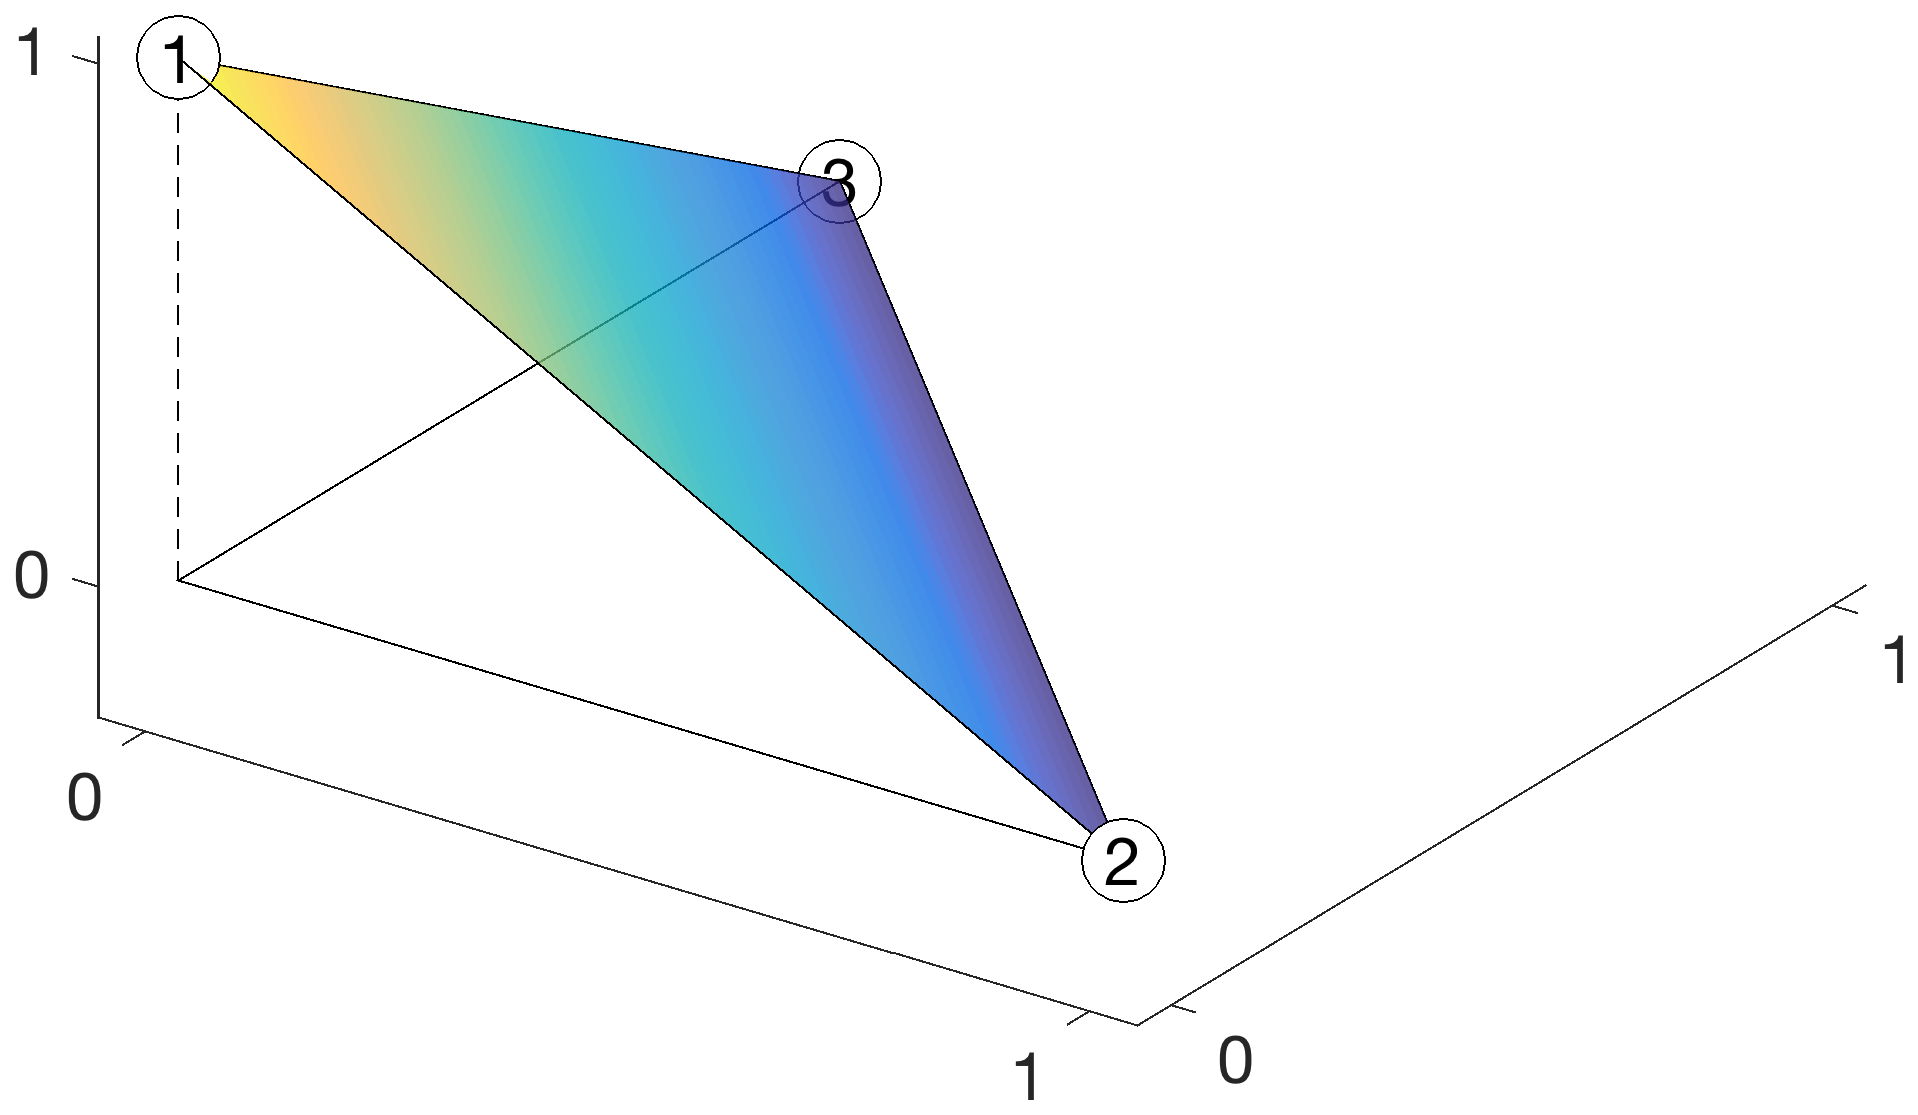
\includegraphics[width=0.3\textwidth]{shape_tri_p1_1}
  }
  \subfigure[$\tilde \phi_2$]{
    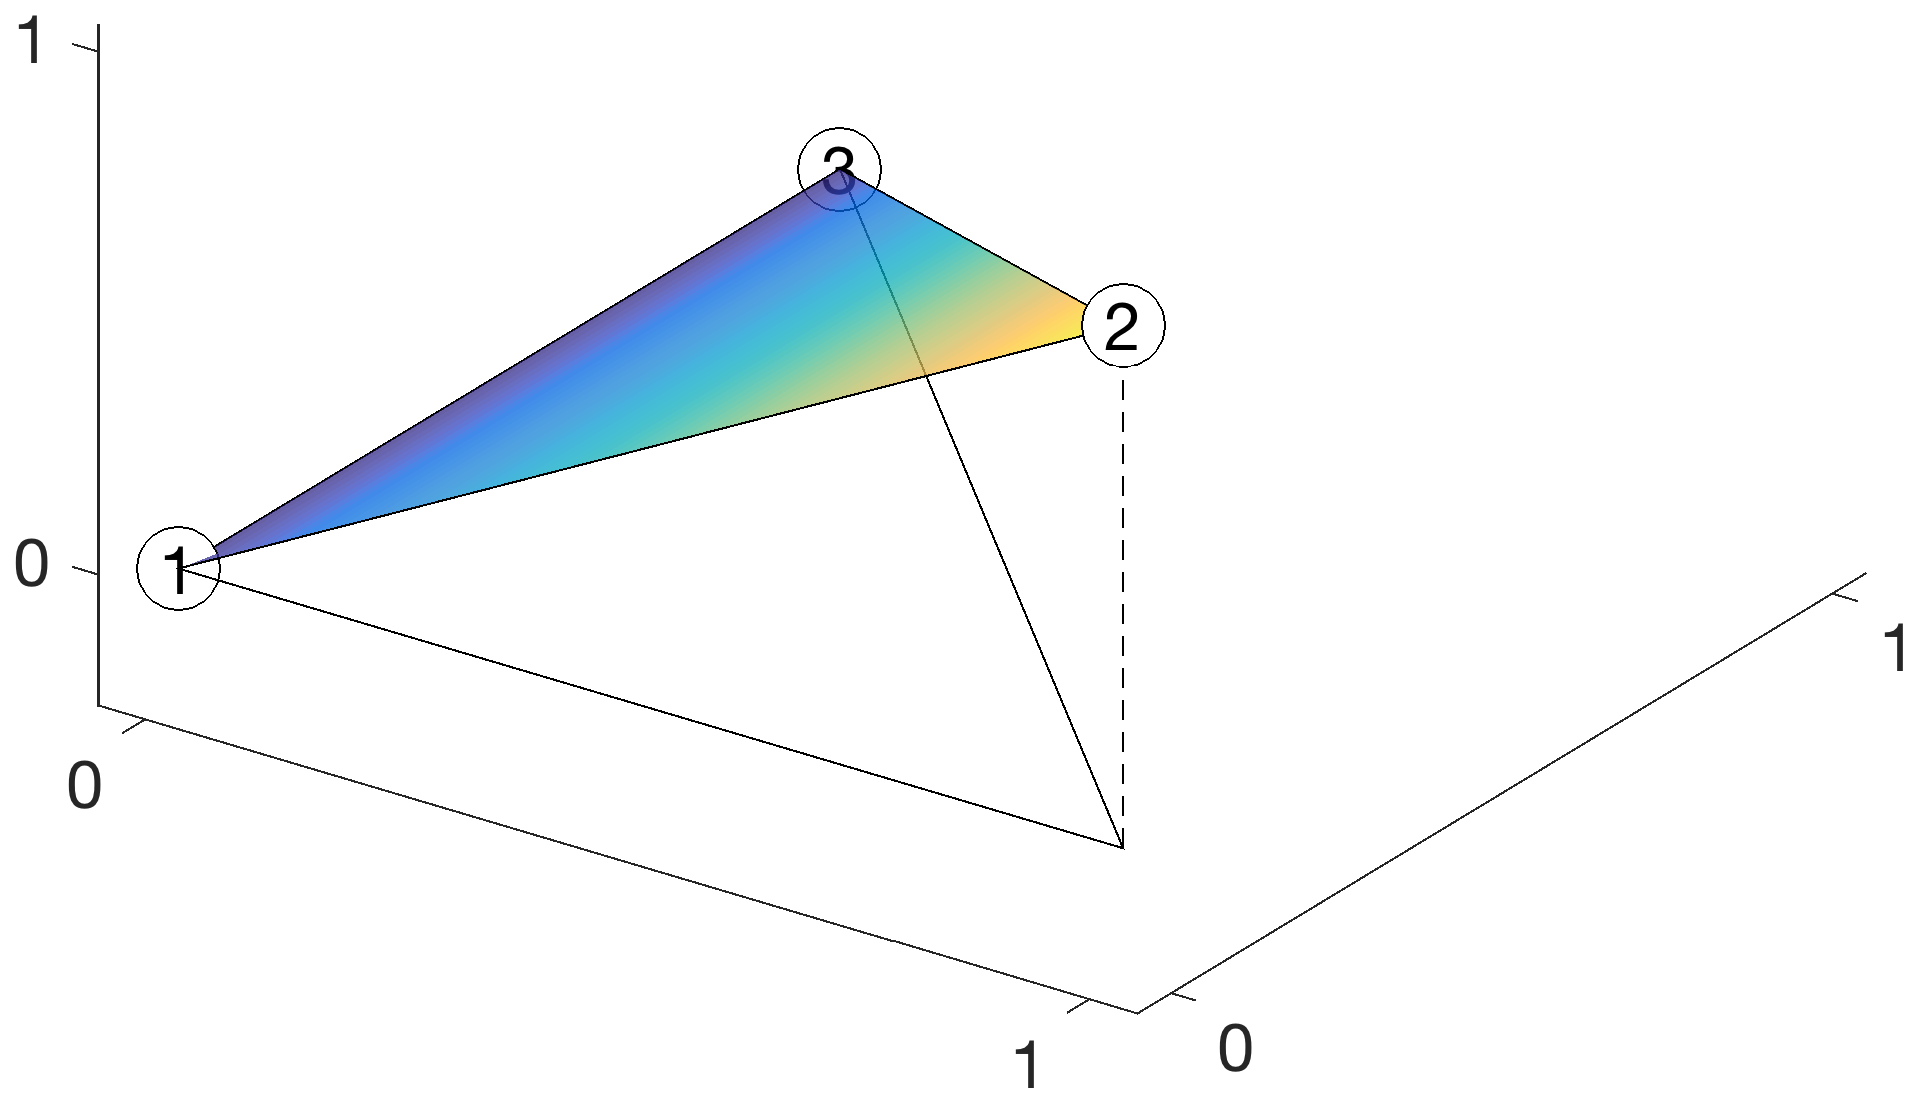
\includegraphics[width=0.3\textwidth]{shape_tri_p1_2}
  }
  \subfigure[$\tilde \phi_3$]{
    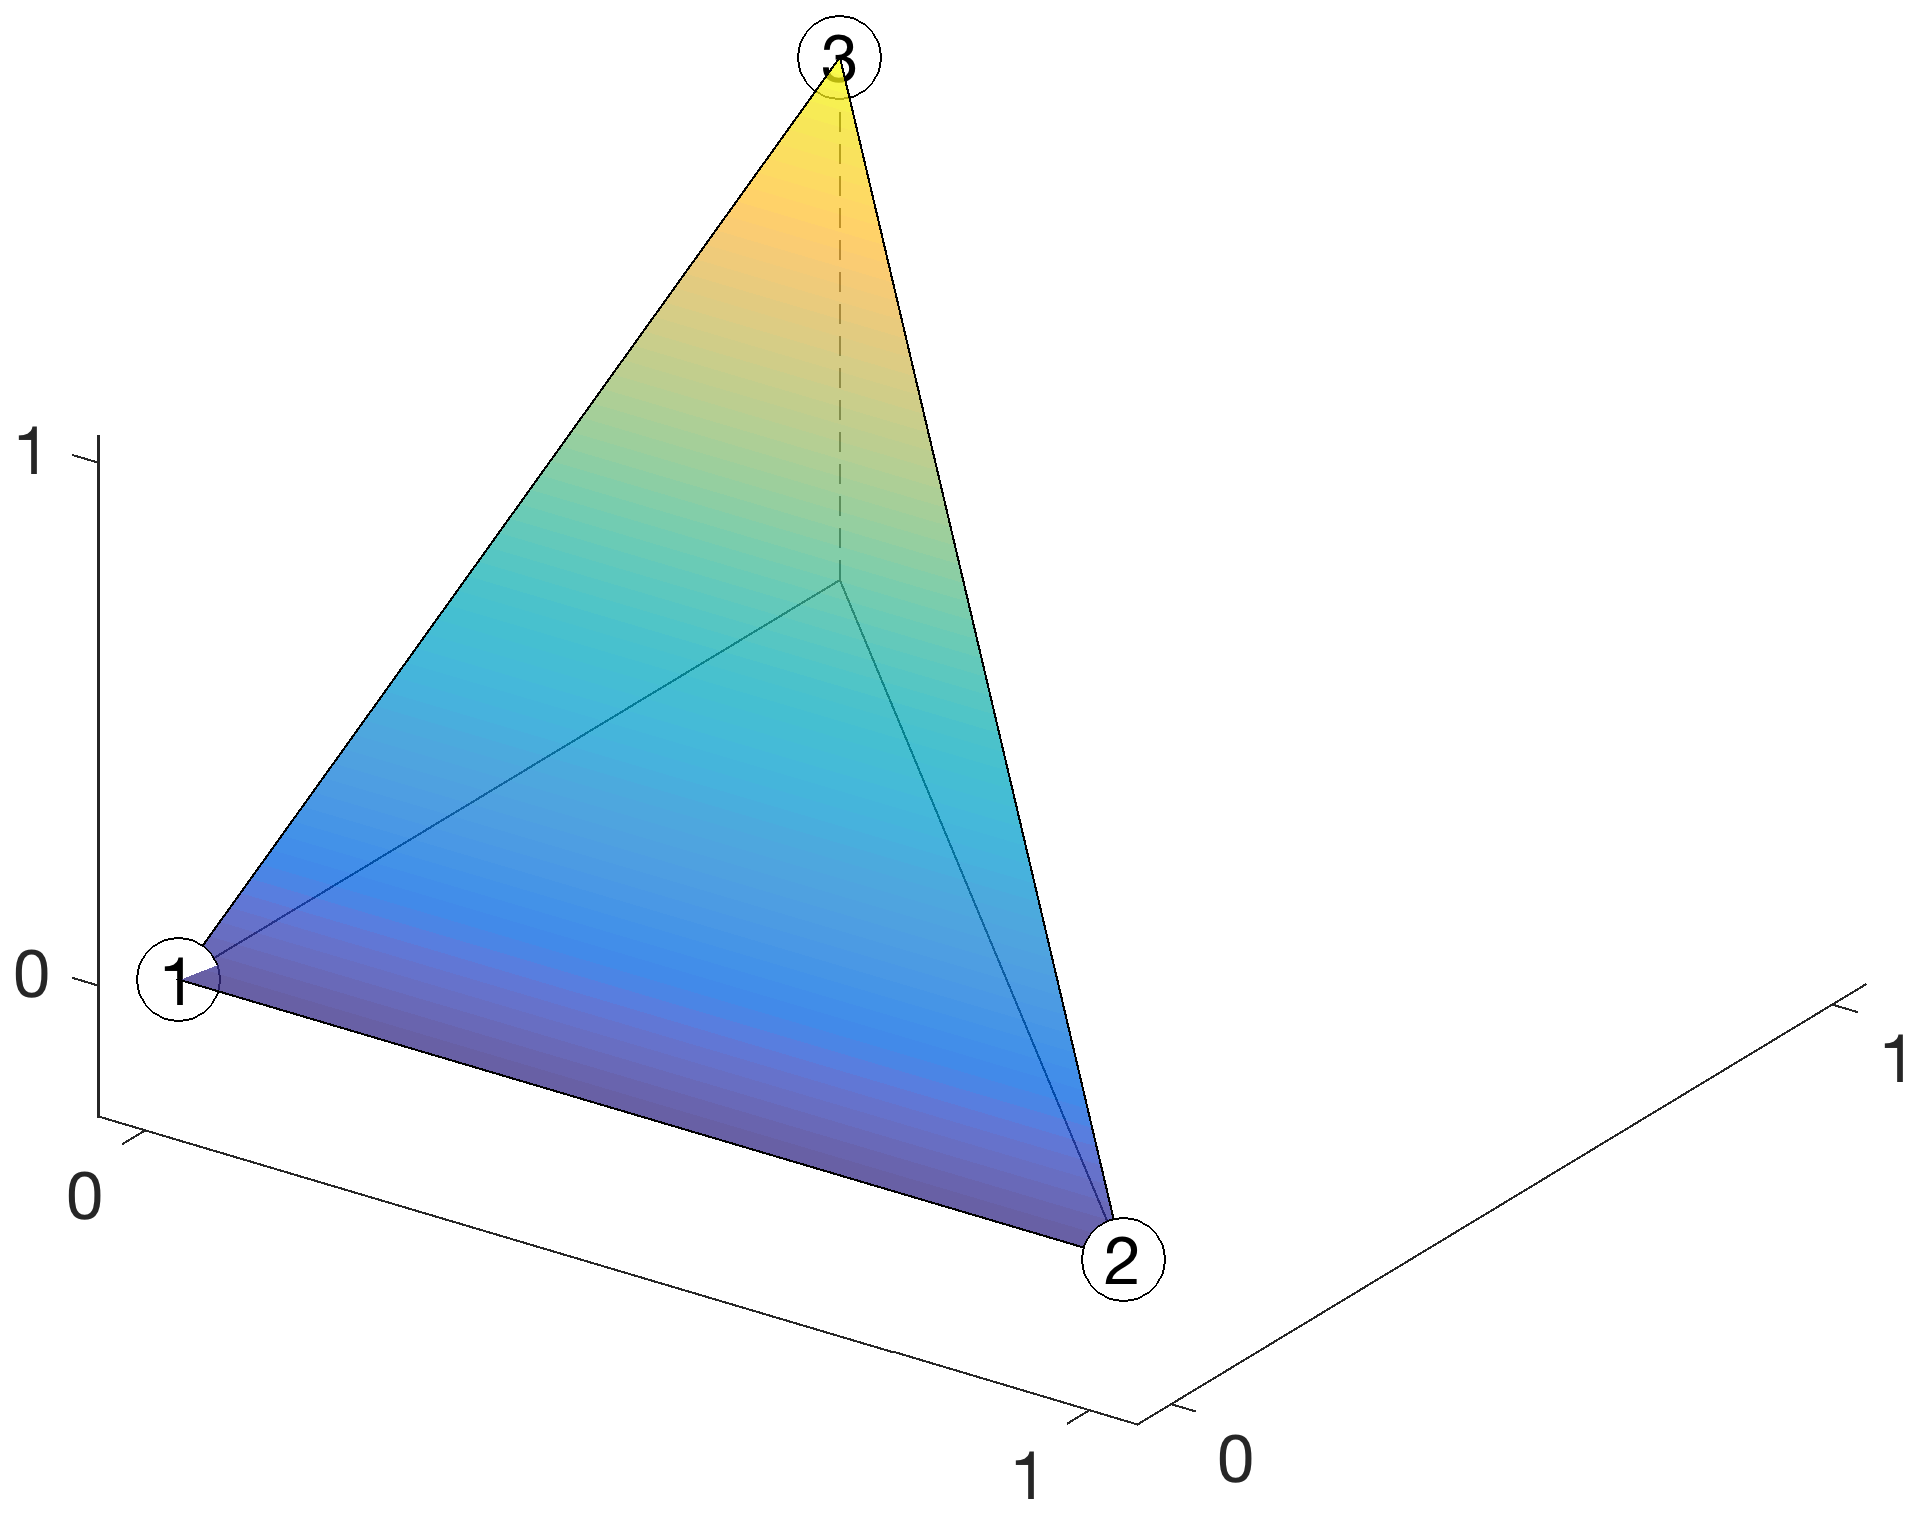
\includegraphics[width=0.3\textwidth]{shape_tri_p1_3}
  }
  \caption{Linear Lagrange shape functions on the reference triangle $\tilde K$.}
  \label{fig:fe_shape_tri_p1}
\end{figure}

Once we find the coefficients of the shape functions, we can evaluate the value of the functions at any point in the triangle by evaluating~\eqref{eq:fe_lin_tri_rep}. We can also differentiate~\eqref{eq:fe_lin_tri_rep} to obtain the gradient of the shape functions:
\begin{equation*}
  \left. \pp{\tilde \phi_j}{\tilde x_1} \right|_{\tilde x} = a_2^{(j)} \quad \text{and} \quad  \left. \pp{\tilde \phi_j}{\tilde x_2} \right|_{\tilde x} = a_3^{(j)}, \quad j = 1,2,3.
\end{equation*}
More explicitly,
\begin{align*}
  \left. \pp{\tilde \phi_1}{\tilde x_1} \right|_{\tilde x} = -1
  \quad &\text{and} \quad
  \left. \pp{\tilde \phi_1}{\tilde x_2} \right|_{\tilde x} = -1\\
  \left. \pp{\tilde \phi_2}{\tilde x_1} \right|_{\tilde x} = 1
  \quad &\text{and} \quad
  \left. \pp{\tilde \phi_2}{\tilde x_2} \right|_{\tilde x} = 0\\
  \left. \pp{\tilde \phi_3}{\tilde x_1} \right|_{\tilde x} = 0
  \quad &\text{and} \quad
  \left. \pp{\tilde \phi_3}{\tilde x_2} \right|_{\tilde x} = 1.
\end{align*}
For the linear Lagrange element, the derivatives are constant (and trivially spans $\PP^0(\tilde K)$).

Before we introduce other finite elements, we use the linear Lagrange element as an example to describe three properties that formally defines a \emph{finite element}:
\begin{enumerate}
\item the domain $\tilde K$ over which the element is defined; e.g., the reference triangle $\tilde K$.
\item the finite-dimensional linear space of functions; e.g., the linear polynomial space $\PP^1(\tilde K)$.
\item the degree of freedom used to describe functions; e.g., the values of the function at the nodes $\{ \tilde z_1, \tilde z_2, \tilde z_3 \}$.
\end{enumerate}





\section{Quadratic Lagrange finite element on a triangle}
We now introduce a quadratic Lagrange finite element on a triangle. A quadratic function in $\PP^2(\tilde K)$ takes on the form $a_1 + a_2 \tilde x_1 + a_3 \tilde x_2 + a_4 \tilde x_1^2 + a_5 \tilde x_1 \tilde x_2 + a_6 \tilde x_2^2$ and has six degrees of freedom; we hence wish to identify a linearly independently set of six quadratic Lagrange basis functions.  To this end, we choose for our Lagrange interpolation nodes the three vertices of the triangle and three points at the middle of the edges,
\begin{equation*}
  \tilde z_1 = (0,0), \quad \tilde z_2 = (1,0), \quad \tilde z_3 = (0,1), \quad \tilde z_4 = (1/2,1/2), \quad \tilde z_5 = (0,1/2), \quad \tilde z_6 = (1/2,0),
\end{equation*}
as shown in Figure~\ref{fig:fe_ref_tri_p2}.  The ordering of the quadratic nodes is not universal in the finite element literature; we here adhere the convention that, for $i \in \{4,5,6\}$, the $i$-th node is on the midpoint of the $(i-3)$-th edge of the reference triangle. Our goal is to find the Lagrange basis functions $\{\tilde \phi_i\}_{i=1}^6$ that lie in the $\PP^2(\tilde K)$ space and satisfy the interpolation condition $\tilde \phi_i(\tilde z_j) = \delta_{ij}$.

\begin{figure}
  \centering
  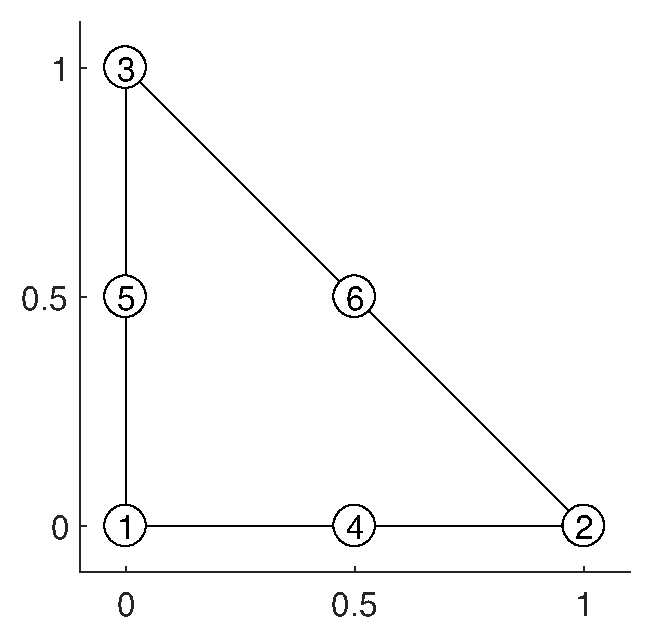
\includegraphics[width=0.3\textwidth]{ref_tri_p2}
  \caption{Quadratic Lagrange finite element on the reference triangle.}
  \label{fig:fe_ref_tri_p2}
\end{figure}


We now employ the procedure used in Section~\ref{sec:fe_lin_tri} to generate the quadratic Lagrange basis. We first express the basis functions in terms of the monomial basis
\begin{equation}
  \tilde \phi_j(\tilde x) = c_1^{(j)} + c_2^{(j)} \tilde x_1 + c_3^{(j)} \tilde x_2 + c_4^{(j)} \tilde x_1^2 + c_5^{(j)} \tilde x_1 \tilde x_2 + c_6^{(j)} \tilde x_2^2 \quad j = 1,\dots,6;
  \label{eq:fe_quad_tri_rep}
\end{equation}
we then express the interpolation condition $\tilde \phi_i(\tilde z_j) = \delta_{ij}$ as a $6 \times 6$ matrix system
\begin{equation*}
  V C = I,
\end{equation*}
where $C_{ij} = c^{(j)}_i$, $i,j = 1,\dots,6$, and the $i$-th row of the Vandermonde matrix $V \in \RR^{6 \times 6}$ is
\begin{equation*}
  V_{i:} = \bmat{cccccc} 1 & \tilde z_{i,1} & \tilde z_{i,2} &  (z_{i,1})^2 & \tilde z_{i,1} \tilde z_{i,2} & (\tilde z_{i,2})^2 \emat .
\end{equation*}
The matrix $V$ is non-singular, and the linear system has a unique solution: $C = V^{-1}$.  Figure~\ref{fig:fe_shape_tri_p2} shows the six basis functions.

\begin{figure}
  \centering
  \subfigure[$\tilde \phi_1$]{
    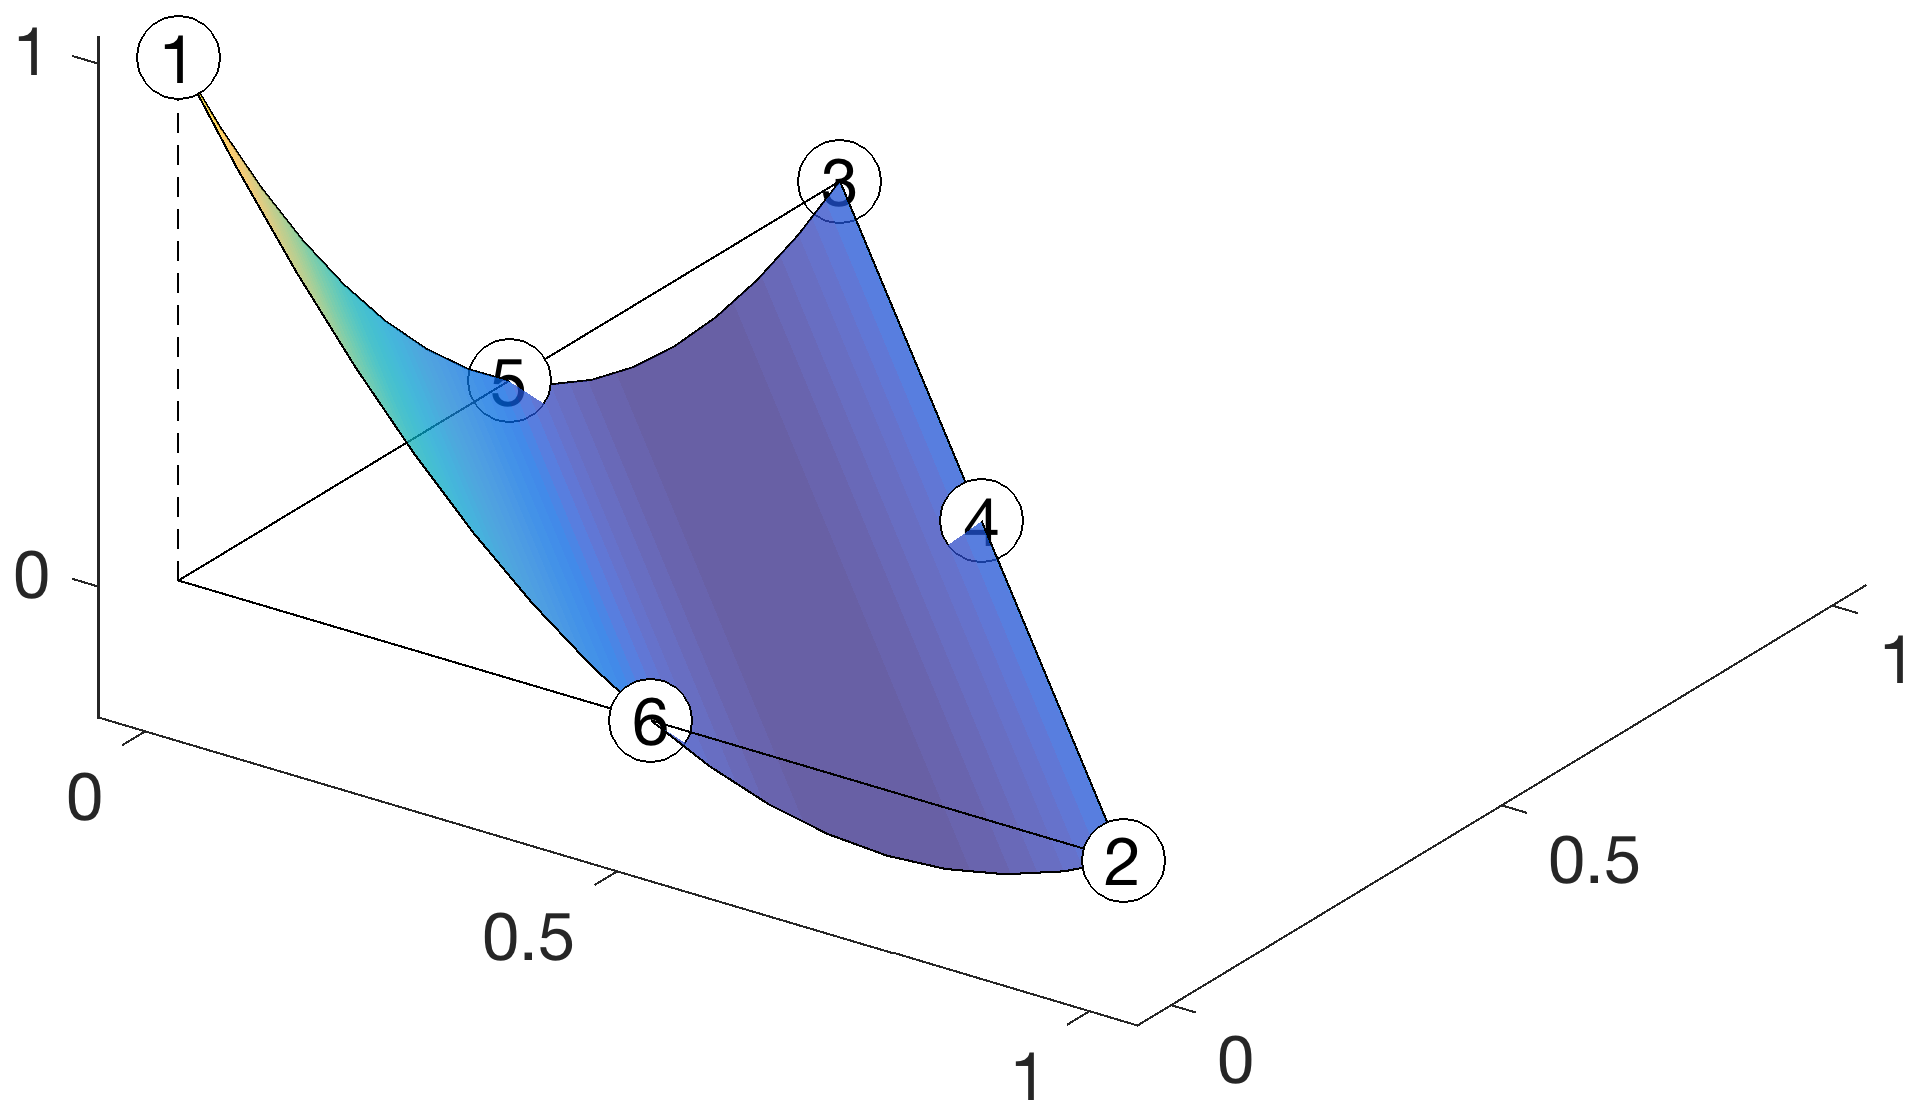
\includegraphics[width=0.3\textwidth]{shape_tri_p2_1}
  }
  \subfigure[$\tilde \phi_2$]{
    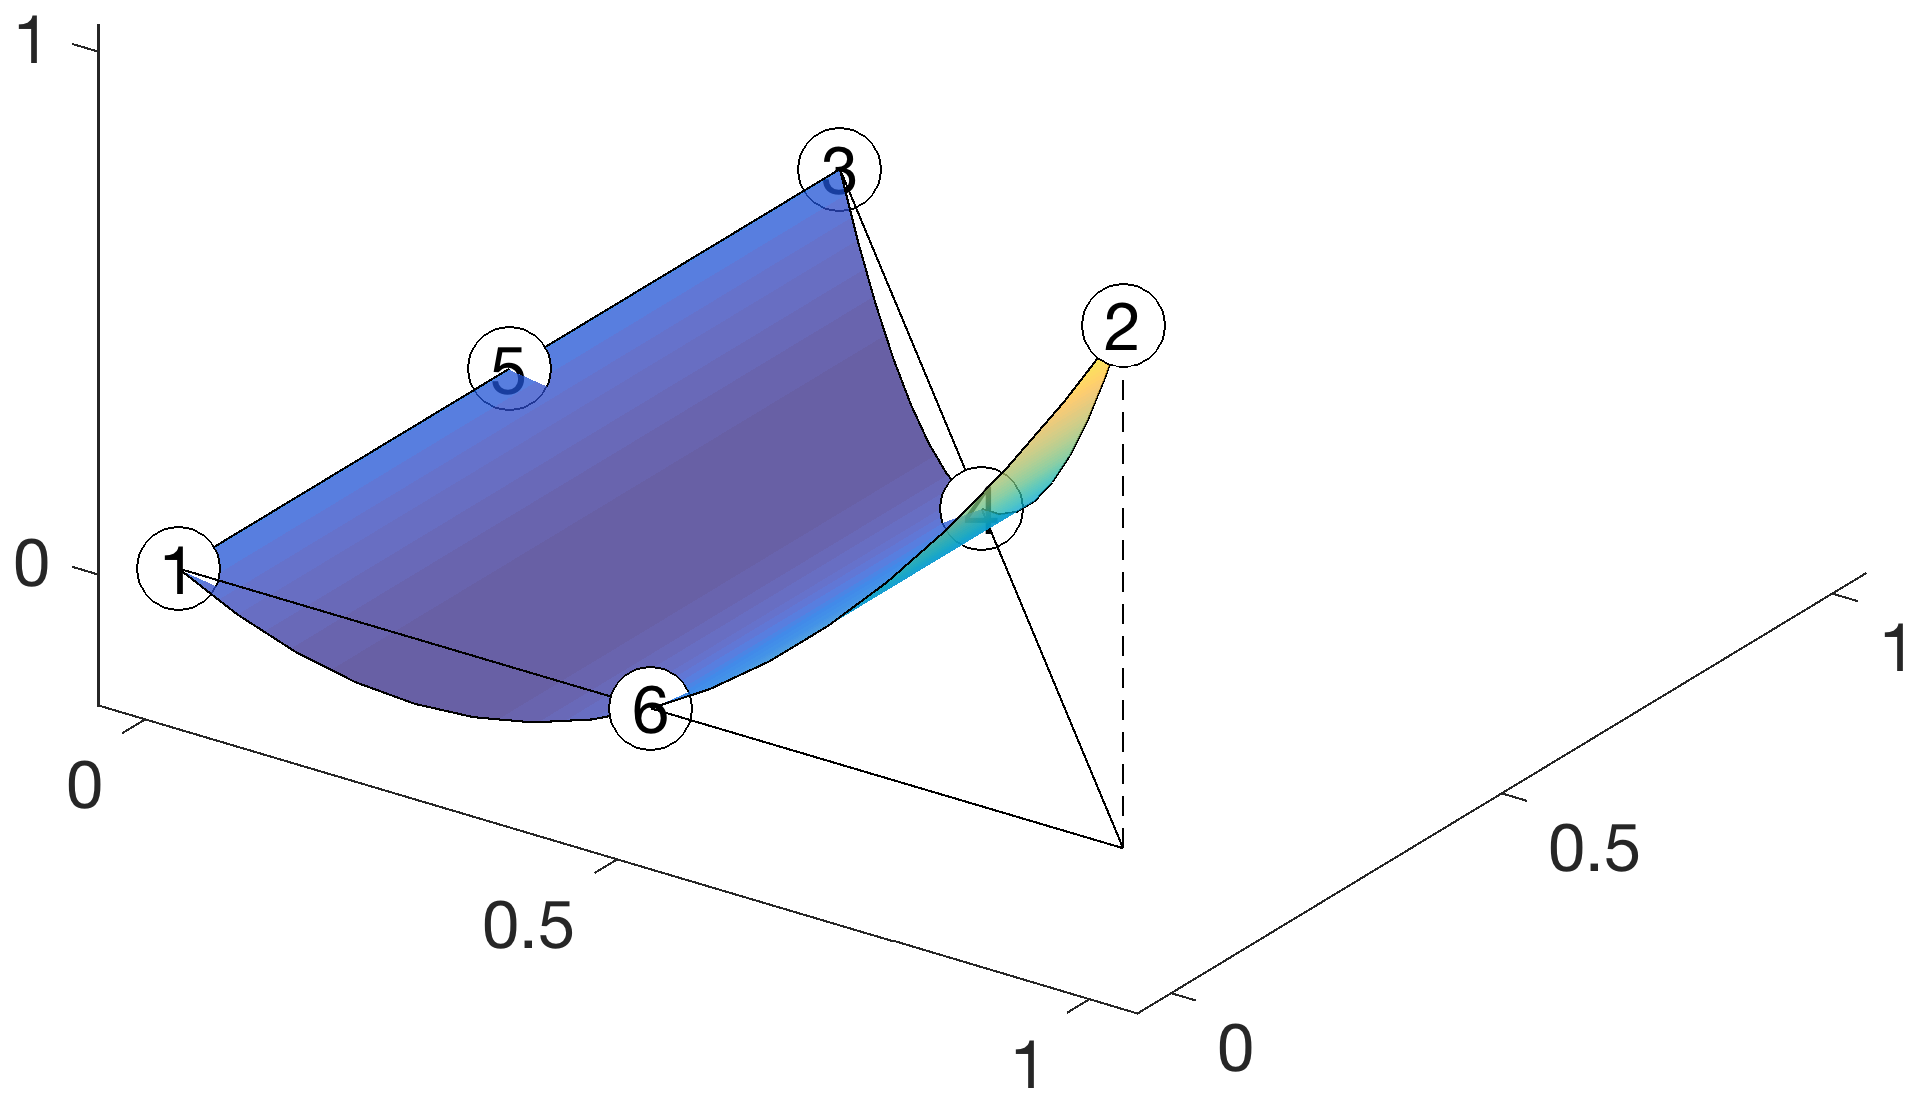
\includegraphics[width=0.3\textwidth]{shape_tri_p2_2}
  }
  \subfigure[$\tilde \phi_3$]{
    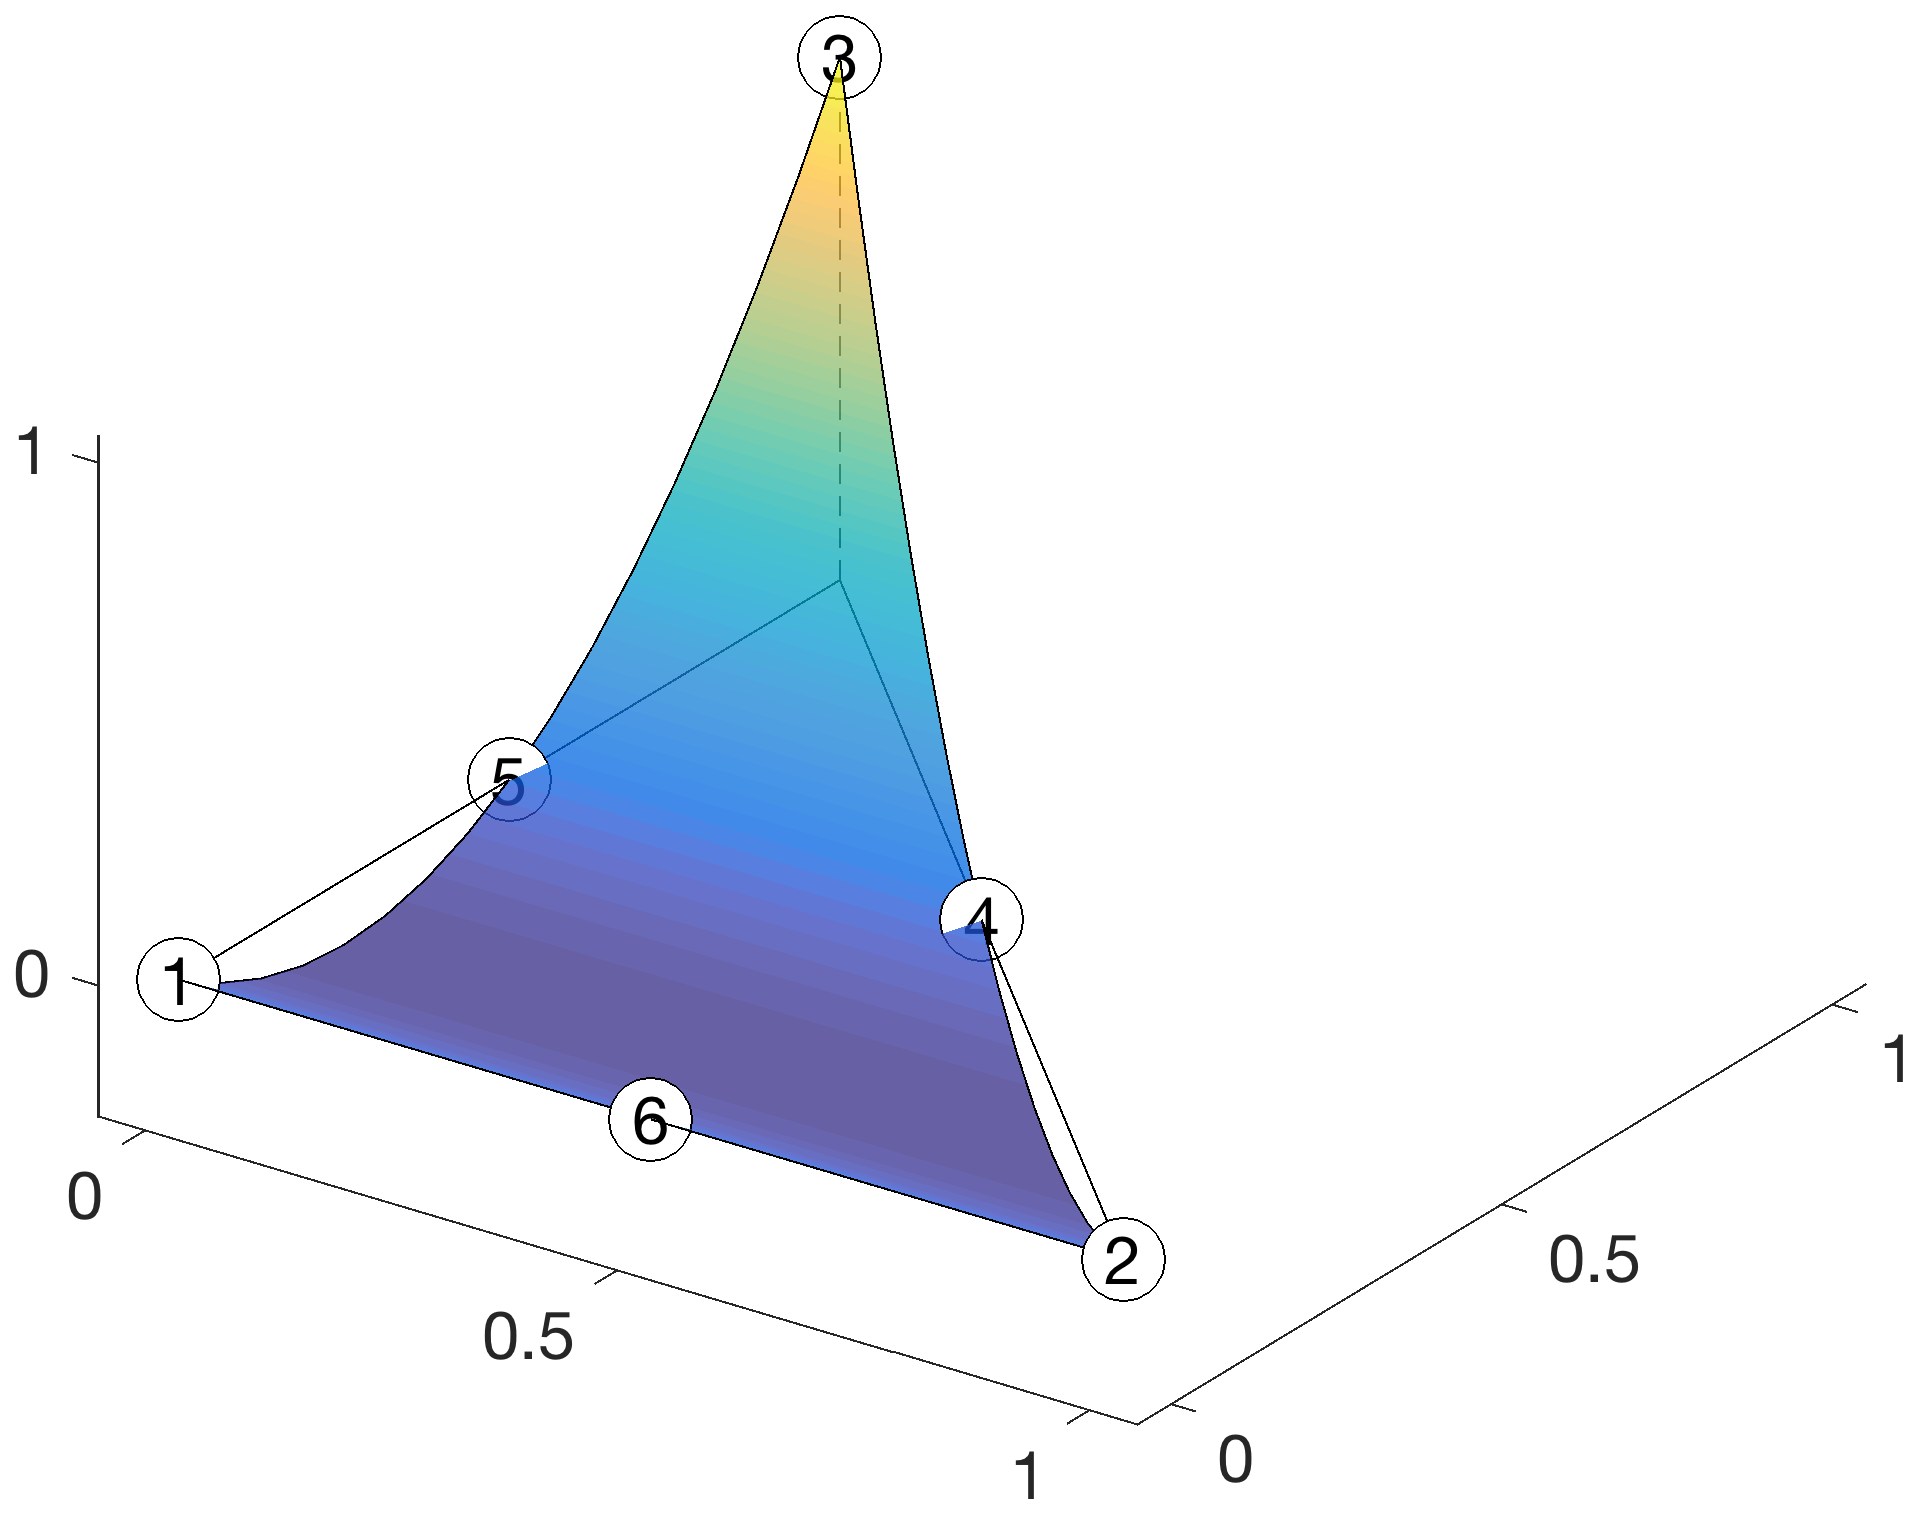
\includegraphics[width=0.3\textwidth]{shape_tri_p2_3}
  }
  \subfigure[$\tilde \phi_4$]{
    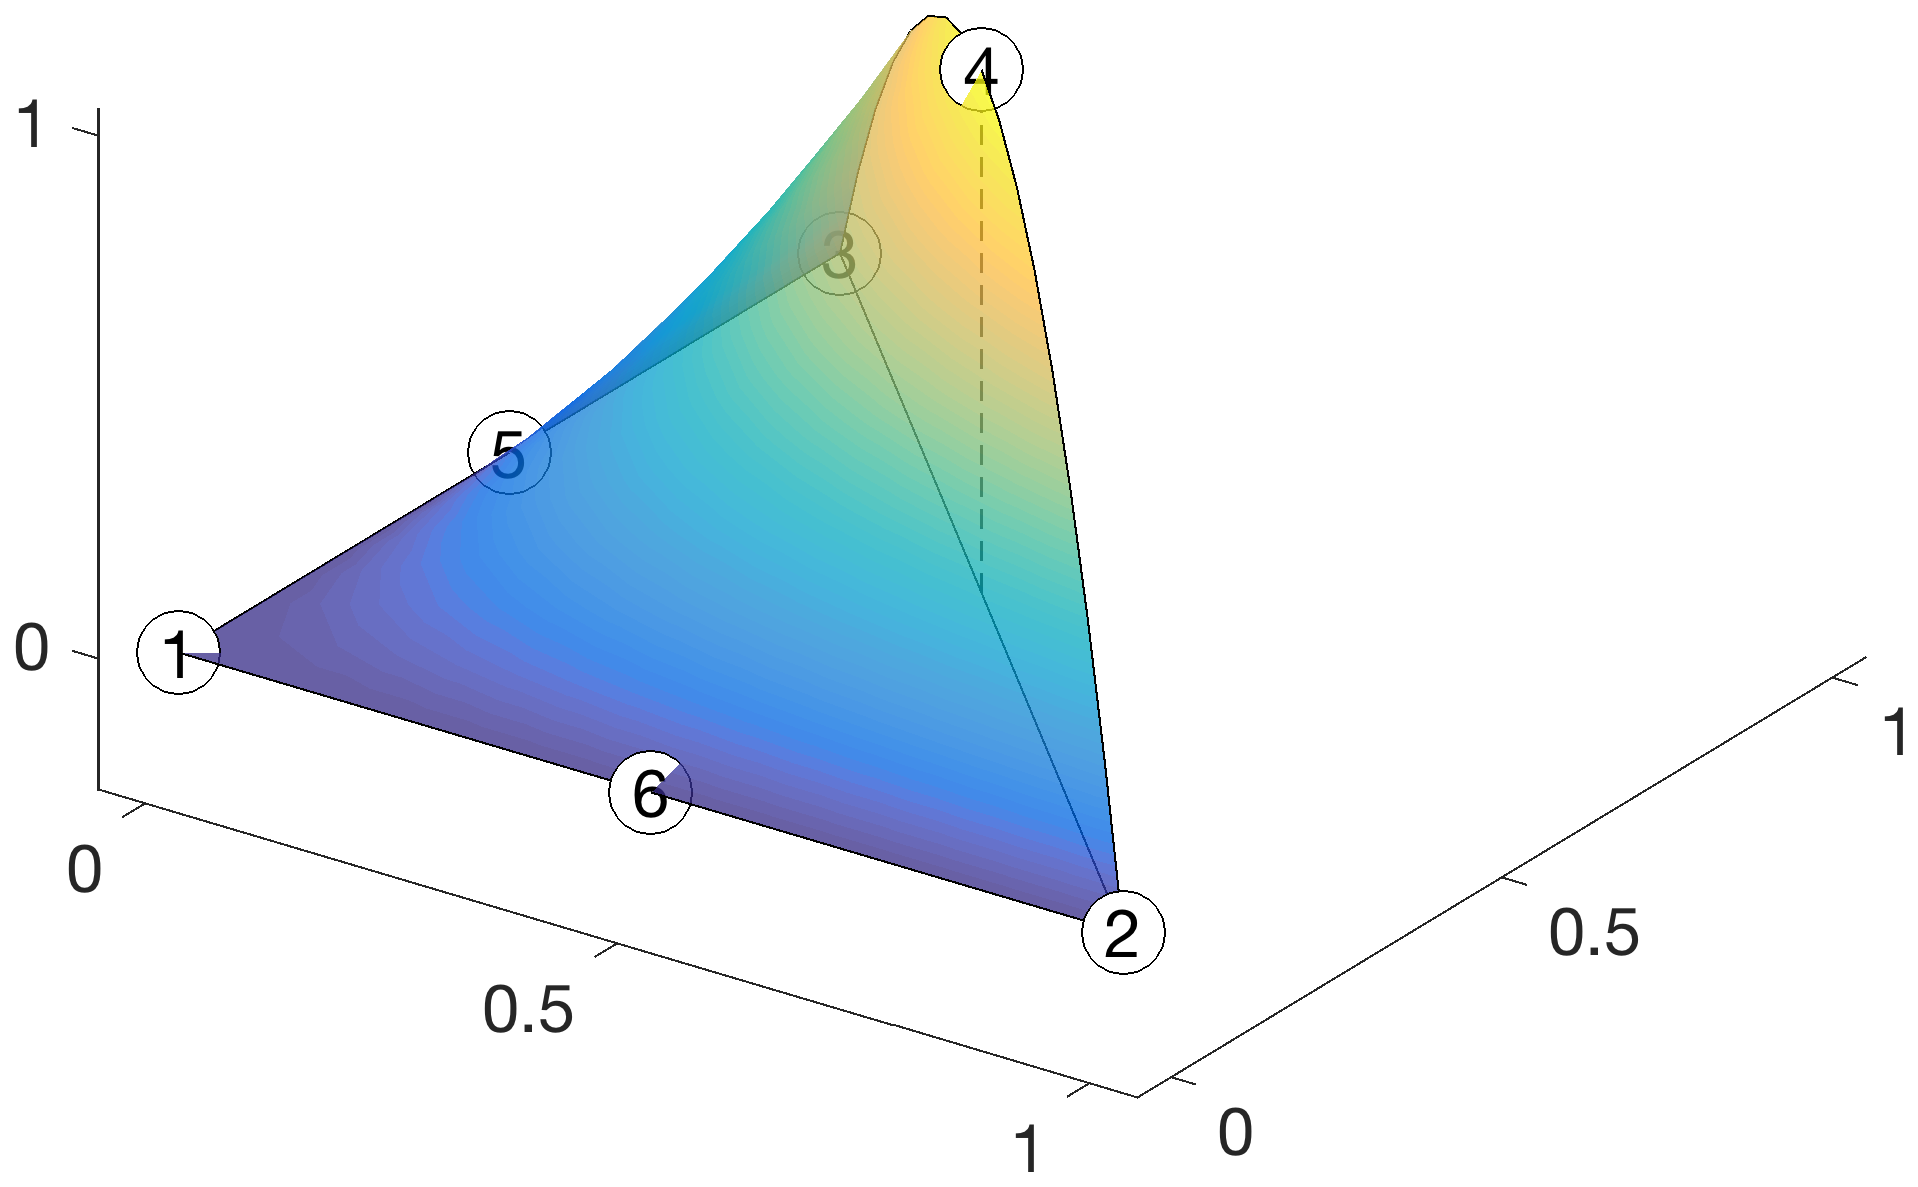
\includegraphics[width=0.3\textwidth]{shape_tri_p2_4}
  }
  \subfigure[$\tilde \phi_5$]{
    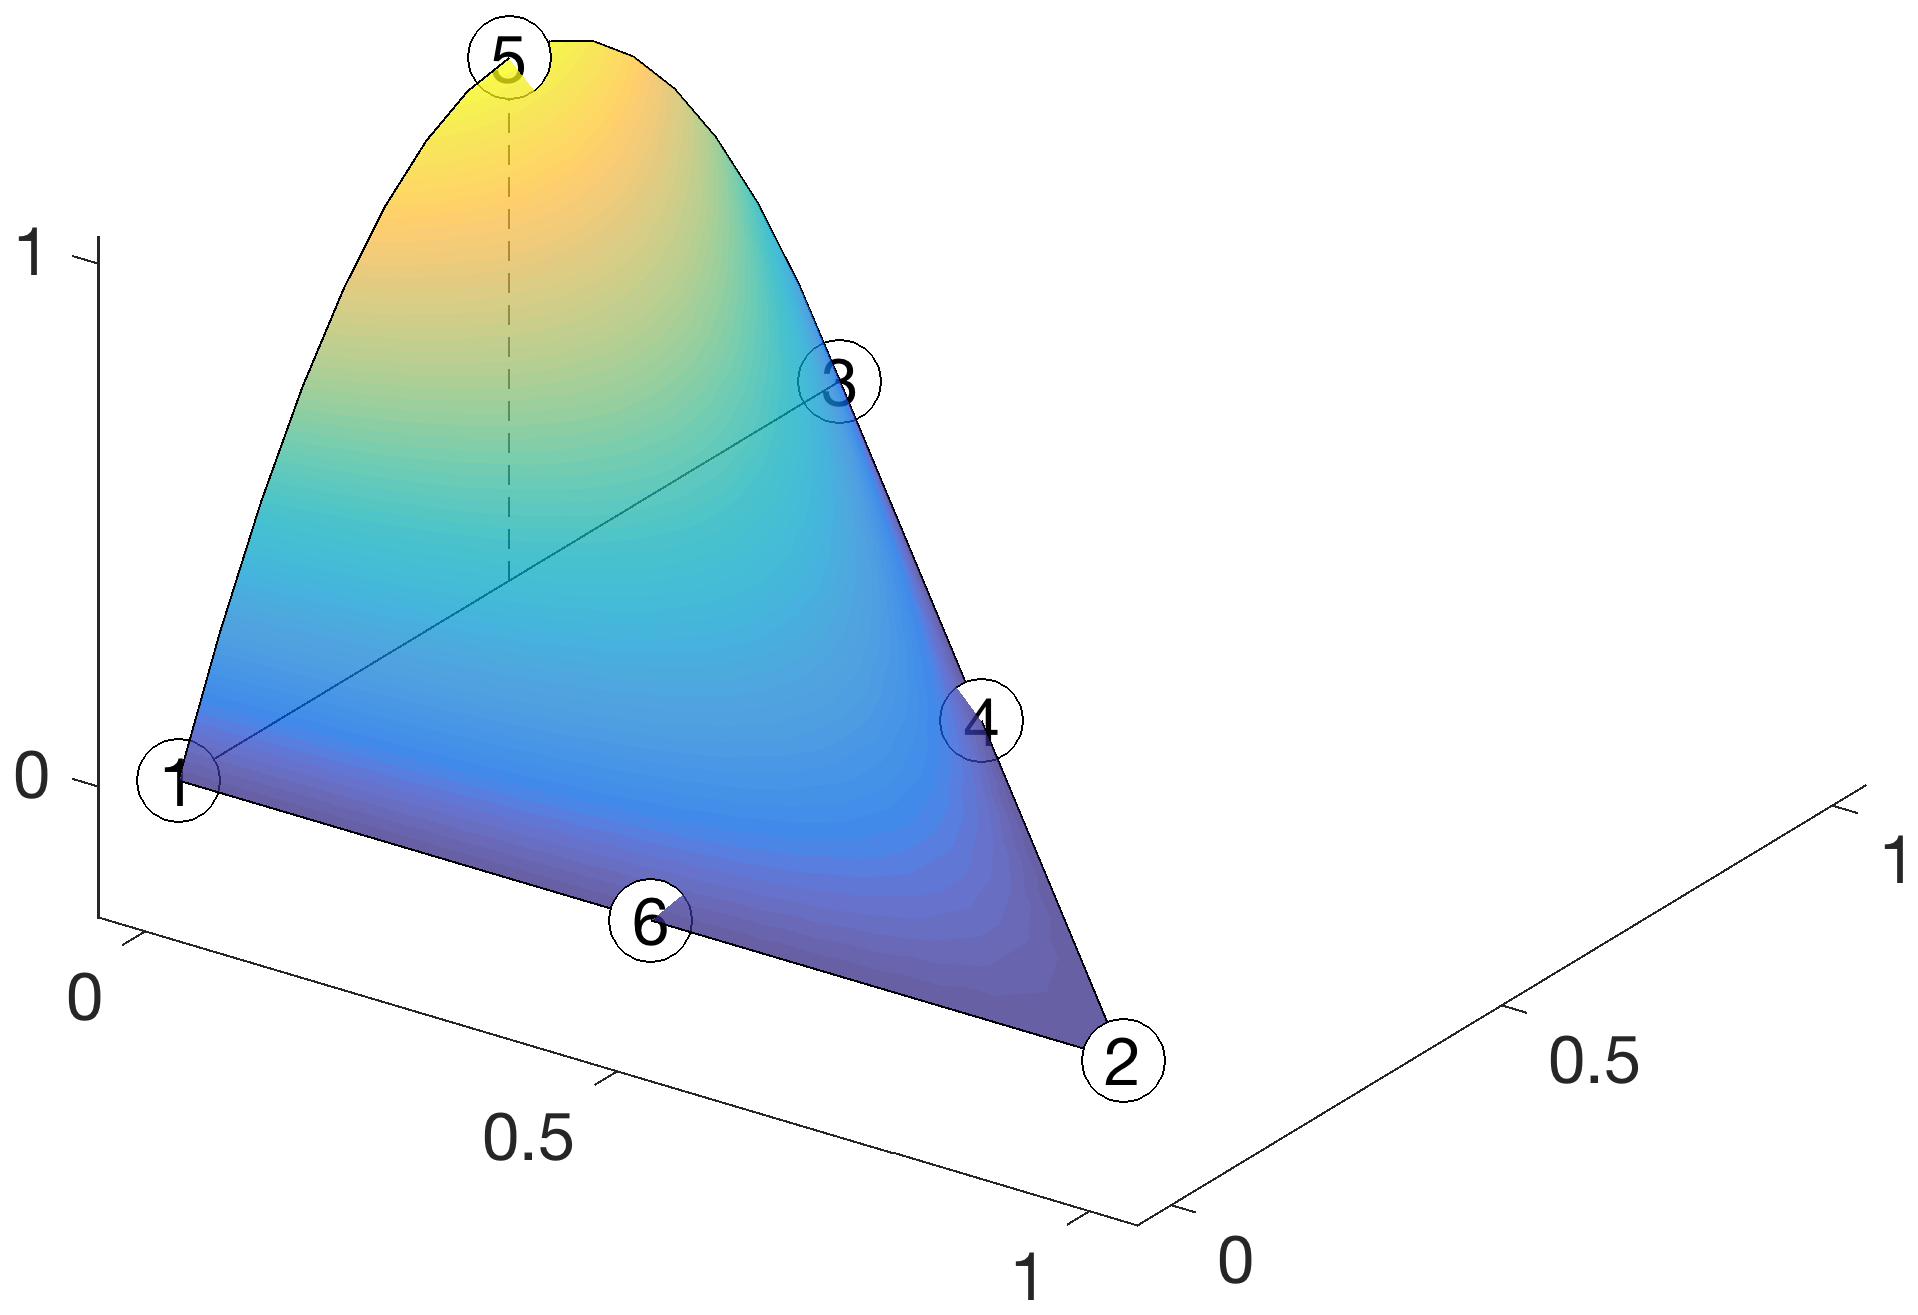
\includegraphics[width=0.3\textwidth]{shape_tri_p2_5}
  }
  \subfigure[$\tilde \phi_6$]{
    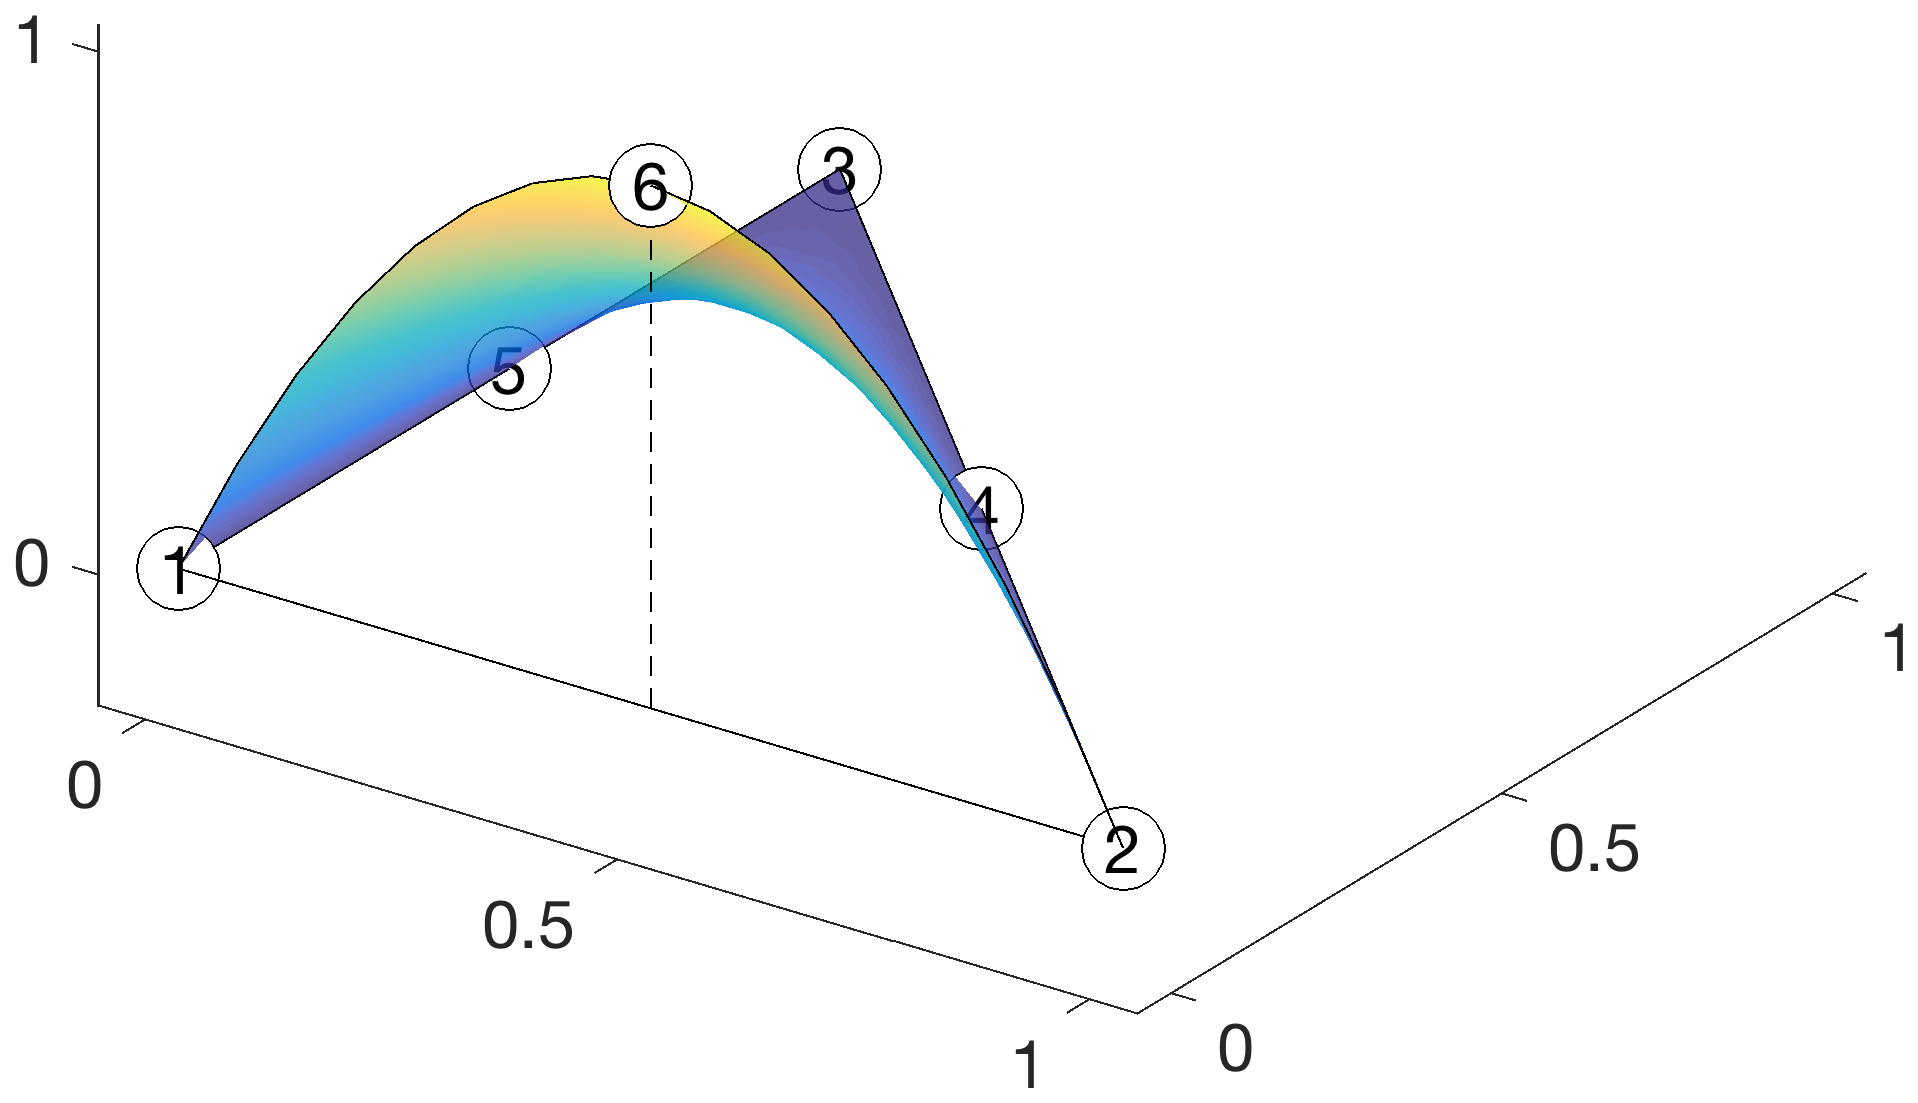
\includegraphics[width=0.3\textwidth]{shape_tri_p2_6}
  }
  \caption{Quadratic Lagrange shape functions on the reference triangle.}
  \label{fig:fe_shape_tri_p2}
\end{figure}

Once we find the coefficients of the basis functions, we can evaluate~\eqref{eq:fe_quad_tri_rep} to obtain the value of the basis function at any point in the reference triangle.  We can also differentiate~\eqref{eq:fe_quad_tri_rep} to obtain the gradient of the shape functions:
\begin{align*}
  \left. \pp{\tilde \phi_j}{\tilde x_1} \right|_{\tilde x} &= c^{(j)}_2 + 2 c^{(j)}_4 \tilde x^2_1 + c^{(j)}_5 \tilde x_2
  \\
  \left. \pp{\tilde \phi_j}{\tilde x_2} \right|_{\tilde x}&= c^{(j)}_3 + c^{(j)}_5 \tilde x_1 + 2 c^{(j)}_6 \tilde x_2.
\end{align*}
For the quadratic Lagrange element, the derivatives are linear functions, and they span $\PP^1(\tilde K)$.

\section{Generation: Lagrange element of arbitrary degree on arbitrary domain}
We can generalize the procedure to generate Lagrange basis functions of an arbitrary degree on an arbitrary domain.  Say we wish to generate Lagrange basis for a polynomial space of degree $p$ with a dimension of $n_s$.  Then, we first identify \emph{any} basis 
\begin{align*}
  \tilde \phi_i = \sum_{j=1}^{n_s} c_i \psi_j
\end{align*}

\begin{align*}
  \bmat{ccc}
  \psi_1(\tilde x^1) & \cdots & \psi_{n_s}(\tilde x^1) \\
  \vdots & \ddots & \vdots \\
  \psi_{n_s}(\tilde x^1) & \cdots & \psi_{n_s}(\tilde x^{n_s}) 
  \emat
  \bmat{ccc}
  c^{(1)}_1 & \cdots & c^{(n_s)}_1 \\
  \vdots & \ddots & \vdots \\
  c^{(1)}_{n_s} & \cdots & c^{(n_s)}_{n_s}
  \emat
  =
  I_{n_s},
\end{align*}
where $I_{n_s}$ is the $n_s \times n_s$ identity matrix.



\section{Isoparametric mapping}
We have so far introduced basis functions defined on a reference element $\tilde K$. We now wish to construct basis functions $\{\phi_i\}_{i=1}^n$ which spans the approximation space $\calV_h \subset \calV$.  (Note that the quantities associated with the physical space do not bear tilde ($\tilde \cdot$), unlike those associated with the reference space.)

To begin, we create a one-to-one map from a point $\tilde x$ in the reference element $\tilde K$ to a point $x$ in the physical element $K$.  To this end, we employ an \emph{isoparametric mapping} which maps a point $\tilde x \in \tilde K$ to a point $x \in K$ according to
\begin{equation}
  x(\tilde x) = \sum_{\alpha=1}^{n_s} z^K_\alpha \tilde \phi_\alpha(\tilde x) ,
  \label{eq:fe_iso_map}
\end{equation}
where $z^K_\alpha$ is the coordinate of the $\alpha$-th node of the physical element $K$, and $\tilde \phi_\alpha$ is the Lagrange basis function associated with the $\alpha$-th node of the reference element.  Note that the isoparametric map is a unique polynomial map that maps the Lagrange interpolation points $\{ \tilde z_\alpha \}_{\alpha}^{n_s}$ of the reference element $\tilde K$ to the respective Lagrange interpolation points $\{ z_\alpha \}_{\alpha}^{n_s}$ of the physical element $K$.

We can differentiate the isoparametric map~\eqref{eq:fe_iso_map} to evaluate the Jacobian of the mapping from $\tilde K$ to $K$, $J (\equiv \pp{x}{\tilde x}): \tilde K \to \RR^{n \times n}$, given by
\begin{equation*}
  J_{ij}(\tilde x)
  = \left. \pp{x_i}{\tilde x_j} \right|_{\tilde x}
  = \sum_{\alpha}^{n_s} z^K_\alpha \left. \pp{\tilde \phi_\alpha}{\tilde x_j} \right|_{\tilde x}.
\end{equation*}
If $\{\tilde \phi_\alpha\}_{\alpha=1}^{n_s}$ is a basis for $\PP^p(\tilde K)$, then the Jacobian $J$ is a degree $p-1$ polynomial in $\tilde x$; consequently, if the approximation space is $\PP^1(\tilde K)$, then the Jacobian is constant over $\tilde K$.  The determinant of the Jacobian $\text{det}(J(\tilde x))$ relates the reference area $d \tilde x$ to the physical area $dx$: $\text{det(J)}: \tilde K \to \RR$ such that
\begin{equation*}
  dx = \text{det}(J(\tilde x)) d\tilde x.
\end{equation*}
We can also compute the inverse Jacobian, the Jacobian of the mapping from $K$ to $\tilde K$: 
\begin{equation*}
 \left. \pp{x_i}{\tilde x_j} \right|_{\tilde x} = (J^{-1}(\tilde x))_{ij}.
\end{equation*}
The algebraic inverse of the Jacobian $\pp{x}{\tilde x}$ is the inverse Jacobian.  In general, the inverse Jacobian is a non-polynomial function of $\tilde x$; the exception is when the approximation space is $\PP^1(\tilde K)$ in which ase the inverse Jacobian is constant (since the Jacobian is constant).

Given the isoparametric map $\tilde K \ni \tilde x \mapsto x \in K$, we now introduce physical basis functions $\{ \phi^K_\alpha \}_{\alpha=1}^{n_s}$ associated with the (physical) element $K \in \calT_h$.  We choose the basis functions that satisfy
\begin{equation}
  \phi^K_\alpha(x(\tilde x)) = \tilde \phi_\alpha(\tilde x) \quad \forall \tilde x \in \tilde K, \quad \alpha 1, \dots, n_s,
  \label{eq:fe_impl_phiK}
\end{equation}
where $\tilde x \mapsto x$ is provided by the isoparametric map~\eqref{eq:fe_iso_map}. In words, the physical basis function $\phi^K_\alpha$ evaluated at the physical point $x(\tilde x) \in K$ takes on the same value as the associated reference basis function $\phi_\alpha$ evaluated at the associated reference point $\tilde x \in \tilde K$.  
We can also differentiate~\eqref{eq:fe_impl_phiK} to obtain the derivative of the physical basis functions in the physical space: given any $\tilde x \in \tilde K$, 
\begin{equation}
  \left. \pp{\phi^K_\alpha}{x_i} \right|_{x(\tilde x)} =
  \sum_{j=1}^{d} \left. \pp{\tilde \phi_\alpha}{\tilde x_j} \right|_{\tilde x} \left. \pp{\tilde x_j}{x_i} \right|_{\tilde x}, \quad \alpha = 1,\dots,n_s.
  \label{eq:fe_impl_dphiK}
\end{equation}
Expressions~\eqref{eq:fe_impl_phiK} and \eqref{eq:fe_impl_dphiK} allows us to evaluate the value and gradient, respectively, of the physical basis function $\phi^K_\alpha$ at a physical point $x(\tilde x) \in K$ associated with a select reference point $\tilde x \in \tilde K$; we will soon see this is exactly the capability we need to evaluate stiffness matrices and load vectors.

As an example, consider the triangulation shown in Figure~\ref{fig:fe_impl_mesh_p1}.  The physical element $K_5 \in \calT_h$ is delineated by the nodes
\begin{equation*}
  z^{K_5}_1 = v_6 = (0.28,-0.07), \quad 
  z^{K_5}_2 = v_5 = (-0.21,0.98), \quad \text{and} \quad
  z^{K_5}_3 = v_3 = (-0.29,0.04);
\end{equation*}
we recall that the dot ($\bullet$) in Figure~\ref{fig:fe_mesh_p1} denotes the first vertex of the physical element, and vertices are in the counter-clockwise order. The third reference basis function $\tilde \phi_3$ over $\tilde K$ is shown in Figure~\ref{fig:fe_impl_loc_shape}.  The associated physical basis function $\phi_3^{K_5}$ over $K_5 \in \calT_h$ is shown in Figure~\ref{fig:fe_impl_glob_shape}.  Note that the $\phi_3^{K_5}$ is by definition defined over only $K_5 \subset \Omega$ and not the entire $\Omega$.

\begin{figure}
  \centering
  \subfigure[triangulation]{
    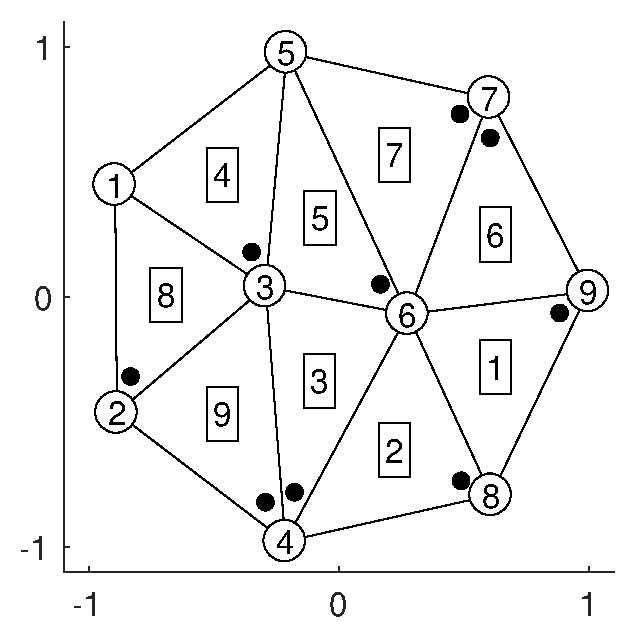
\includegraphics[width=0.3\textwidth]{fe_mesh_p1}
    \label{fig:fe_impl_mesh_p1}
  }
  \subfigure[reference basis function $\tilde \phi_3$]{
    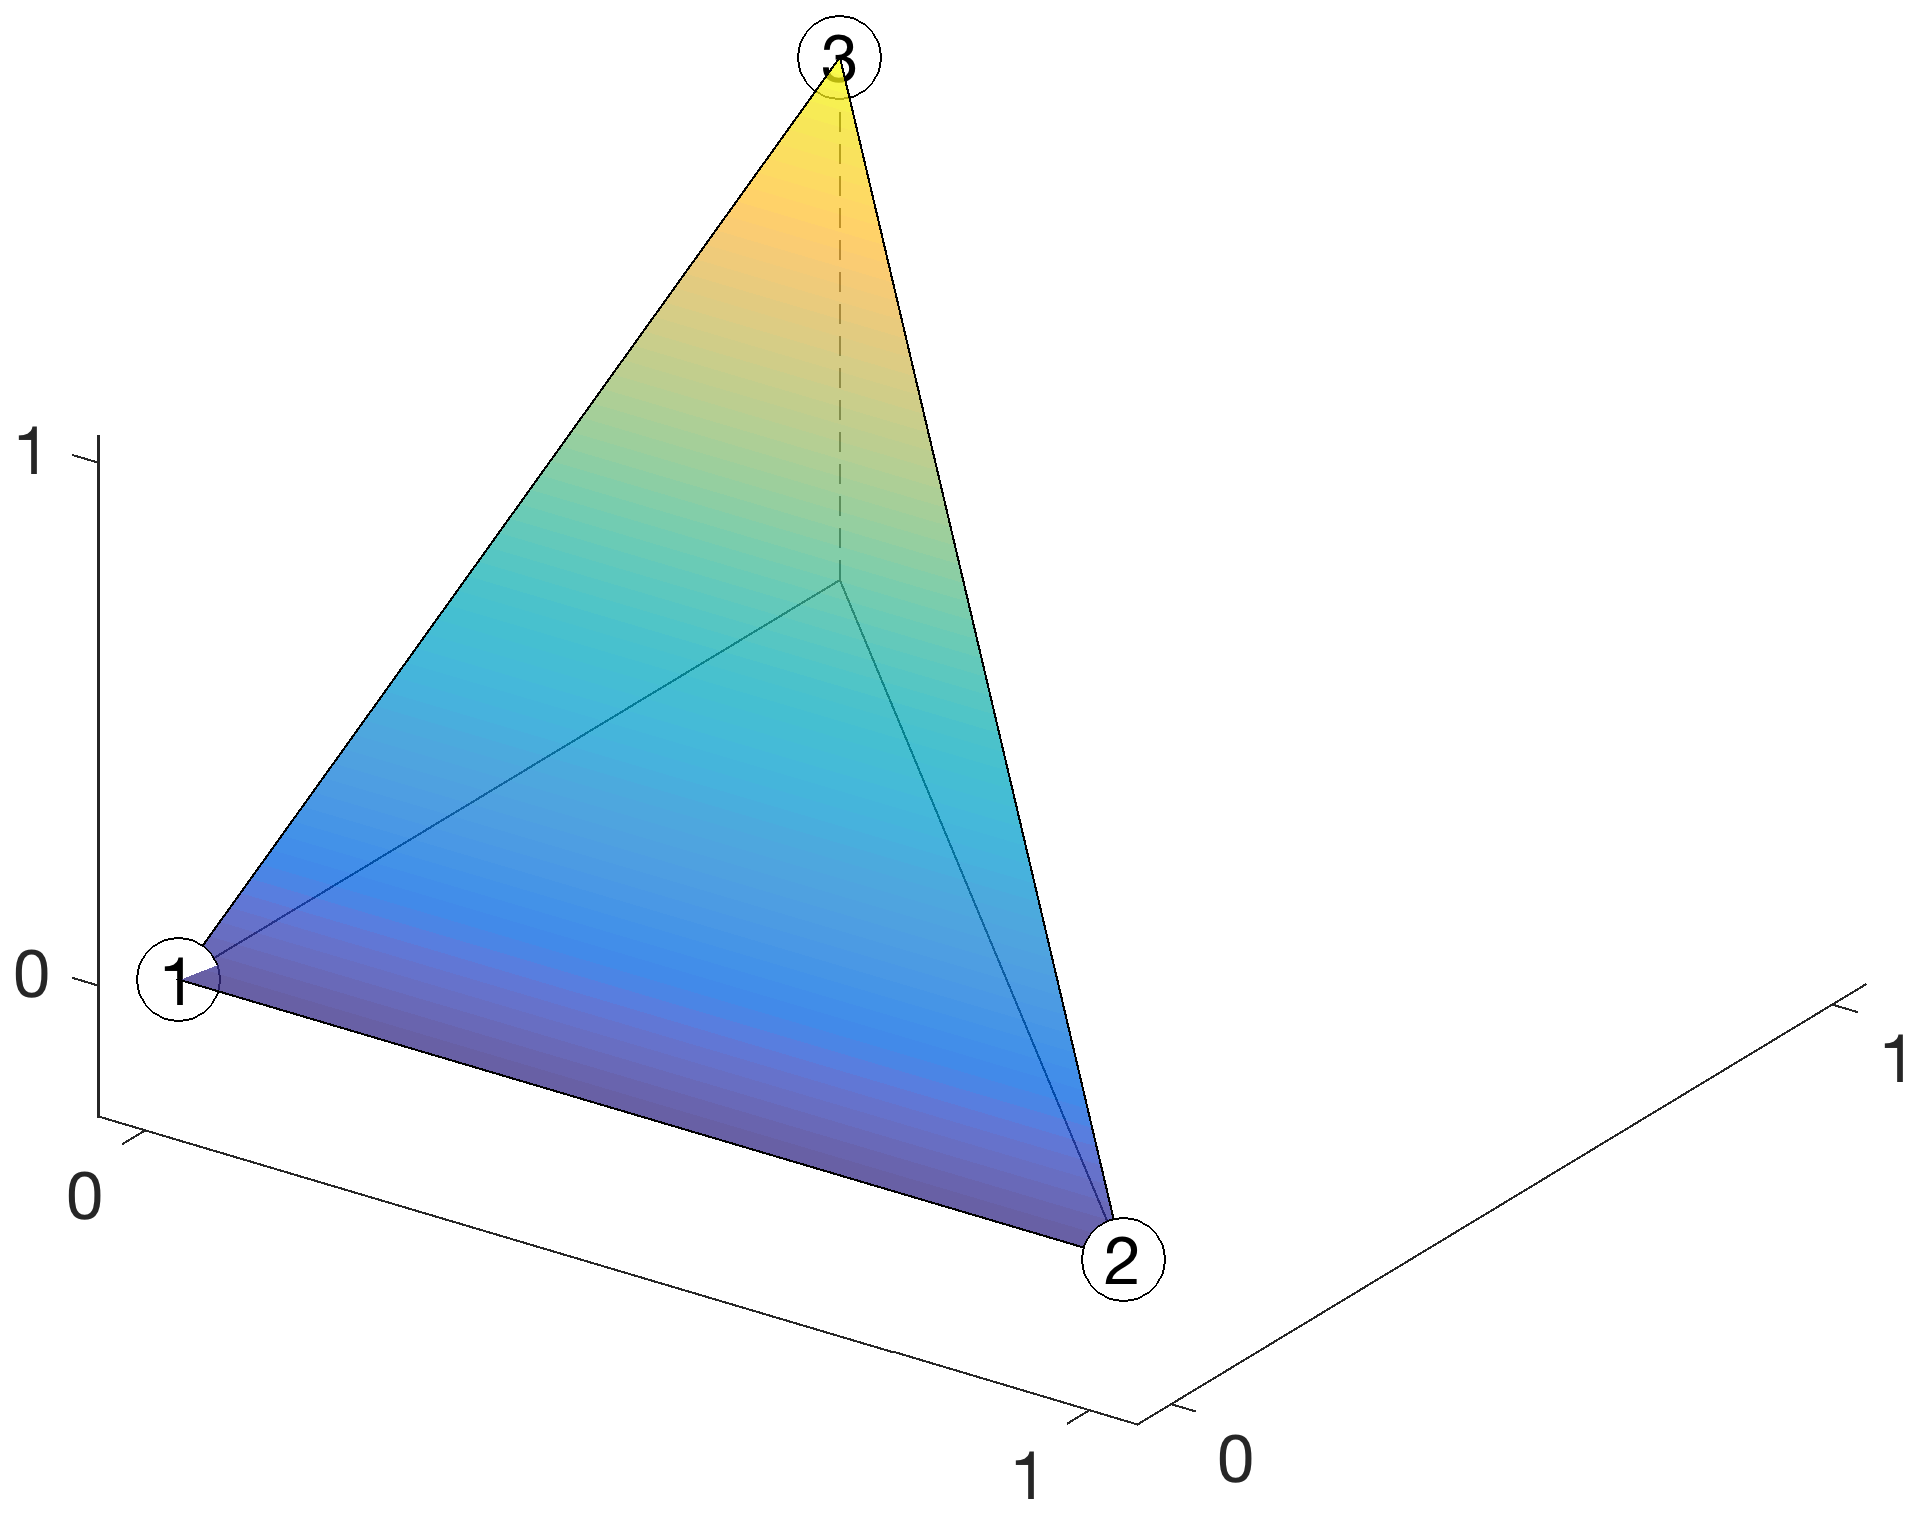
\includegraphics[width=0.3\textwidth]{shape_tri_p1_3}
    \label{fig:fe_impl_loc_shape}
  }
  \subfigure[physical basis function $\phi^{K_5}_3$]{
    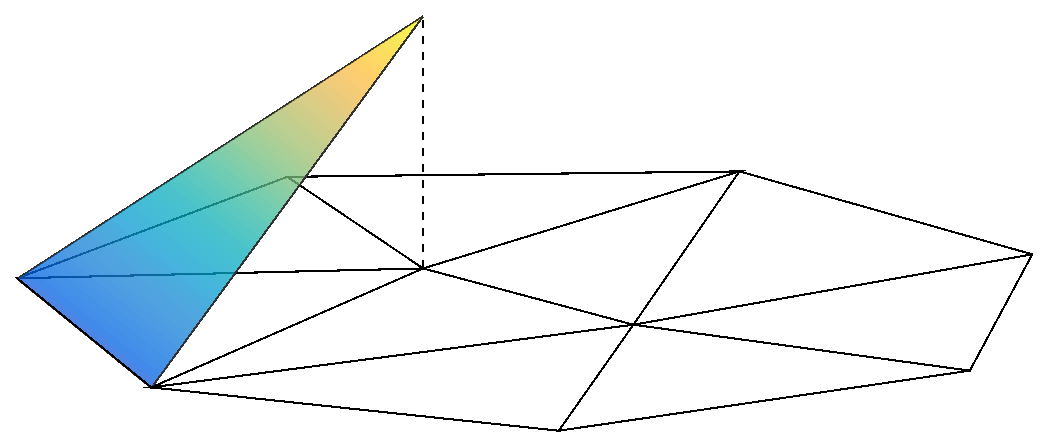
\includegraphics[width=0.33\textwidth]{shape_global_p1_part}
    \label{fig:fe_impl_glob_shape}
  }
\end{figure}


We make one remark about our physical basis functions defined by~\eqref{eq:fe_impl_phiK}.  Even though the reference basis function $\tilde \phi: \tilde K \to \RR$ is a polynomial in $\tilde K$, the physical basis function $\phi^K_\alpha: K \to \RR$ is in general a non-polynomial function in $K$. To see this, we observe that $\phi^K_\alpha(x) = \tilde \phi_\alpha(\tilde x(x))$, $\forall x \in K$; because the inverse map $K \ni x \mapsto \tilde x \in \tilde K$ is not a polynomial in $K$, the function $\phi^K_\alpha(\cdot) = \tilde \phi_\alpha(\tilde x (\cdot))$ is not a polynomial in $K$.  The exception is when the isoparametric mapping is based on the $\PP^1(\tilde K)$ space, in which case the inverse map $K \ni x \mapsto \tilde x \in \tilde K$ is affine and $\phi^K_\alpha(\cdot) = \tilde \phi_\alpha(\tilde x (\cdot))$ is linear in $K$.

Using these basis functions, we can 

given $\tilde x \in \tilde K$,
\begin{equation*}
  v(x(\tilde x))
  %= \tilde v(\tilde x)
  = \sum_{\alpha = 1}^{n_s} \hat v_\alpha \phi^K_\alpha(x(\tilde x))
\end{equation*}
\begin{equation*}
  \left. \pp{v}{x} \right|_{x(\tilde x)} 
  % = \left. \pp{\tilde v}{\tilde x} \right|_{\tilde x} \left. \pp{\tilde x}{x} \right|_{\tilde x}
  = \sum_{\alpha = 1}^{n_s} \hat v_\alpha \left. \pp{\phi^K_\alpha}{x} \right|_{x(\tilde x)}
\end{equation*}


\section{Numerical quadrature}
The entries of the element stiffness matrix $\hat A^K \in \RR^{n_s \times n_s}$ can be expressed as an integral over the reference element $\tilde K$:
\begin{align*}
  \hat A^K_{\alpha\beta}
  &\equiv \int_{K} \left. \pp{\phi_\alpha^K}{x_i} \right|_{x} a_{ij}(x) \left. \pp{\phi_\beta^K}{x_j} \right|_x dx
  \\
  &= \int_{\tilde K} \left. \pp{\phi_\alpha^K}{x_i} \right|_{x(\tilde x)} a_{ij}(x(\tilde x)) \left. \pp{\phi_\beta^K}{x_j} \right|_{x(\tilde x)} \det(J(\tilde x)) d\tilde x , \quad \alpha,\beta = 1,\dots,n_s.
\end{align*}
So far in this lecture we have introduced the means to evaluate all the terms that appear in the integrand --- $\left. \pp{\phi_\alpha^K}{x_i} \right|_{x(\tilde x)}$, $a_{ij}(x(\tilde x))$, and $\text{det}(J(\tilde x))$.  The last ingredient we need is a means to evaluate the integral over $\tilde K$ from a finite evaluation of the integrand.

We now introduce \emph{numerical quadrature} (or just \emph{quadrature}) to perform the integration.  Specifically, our quadrature problem is as follows: given $f: \tilde K \to \RR$, estimate the integral
\begin{equation*}
  I \equiv \int_{\tilde K} f(\tilde x) d \tilde x
\end{equation*}
by
\begin{equation*}
  Q \equiv \sum_{q=1}^{n_q} \tilde \rho_q f(\tilde \xi_q),
\end{equation*}
where $\{\tilde \xi_q \in \tilde K \}_{q=1}^{n_q}$ is a set of \emph{quadrature points} and $\{\tilde \rho_q \in \RR \}_{q=1}^{n_q}$ is the associated set of \emph{quadrature weights}.

\section{Gauss quadrature in $\RR^1$}
We first consider a one-dimensional quadrature for a unit line segment $\tilde I \equiv (0,1) \subset \RR^1$.  (Note: one-dimensional quadrature rules are often defined for the line segment $(-1,1)$; in this lecture we define them for $(0,1)$ to be consistent with our definition of a unit line segment.)  While there are many one-dimensional quadrature rule, we focus here on arguably the most efficient quadrature rule: the Gauss quadrature.

The $n_q$-point Gauss quadrature rule is defined by quadrature points $\{\tilde \xi_q \in \tilde I \}_{q=1}^{n_q}$ and quadrature weights $\{ \tilde \rho_q \in \tilde I \}_{q=1}^{n_q}$ such that the rule integrates exactly polynomials of degrees up to and including $2n_q - 1$: i.e.,
\begin{equation}
  \int_{\tilde I} f(\tilde x) d\tilde x = \sum_{q=1}^{n_q} \tilde \rho_q f(\tilde \xi_q) \quad \forall f \in \PP^{2n_q-1}(\tilde I).
  \label{eq:fe_impl_gauss_cond}
\end{equation}
Our intuition might suggest the existence of a $n_q$-point quadrature rule that integrates exactly polynomials of degree $2n_q-1$, as the polynomials have $2n_q$ degrees of freedom and the quadrature rule also has $2n_q$ degrees of freedom --- $n_q$ points and $n_q$ weighs.


We can show the existence of such a rule in a constructive manner using the scaled Legendre polynomials $\{ \tilde \psi_i \}$. (Our Legendre polynomials are scaled such that they are orthogonal over with respect to $L^2(\tilde I \equiv (0,1))$ instead of the usual $L^2((-1,1))$.) The quadrature points $\{ \tilde \xi_q \}_{q=1}^{n_q}$ are the roots of the degree $n_q$ Legendre polynomial:
\begin{equation}
  \tilde \psi_{n_q}(\tilde \xi_q) = 0, \quad q = 1,\dots,n_q.
  \label{eq:fe_impl_gauss_points}
\end{equation}
The quadrature weights $\{\tilde \rho_q \}_{q=1}^{n_q}$ are then chosen to satisfy the following linear equation:
\begin{equation}
  \bmat{ccc}
  \tilde \psi_0(\tilde \xi_1) & \dots & \tilde \psi_0(\tilde \xi_{n_q}) \\
  \vdots & \ddots & \vdots \\
  \tilde \psi_{n_q-1}(\tilde \xi_1) & \dots & \tilde \psi_{n_q-1}(\tilde \xi_{n_q}) 
  \emat
  \bmat{c}
  \tilde \rho_1 \\ \vdots \\ \tilde \rho_{n_q}
  \emat
  =
  \bmat{c}
  \int_{\tilde I} \tilde \psi_0(\tilde x) d\tilde x \\
  \vdots \\
  \int_{\tilde I} \tilde \psi_{n_q-1}(\tilde x) d\tilde x
  \emat .
  \label{eq:fe_impl_gauss_weights}
\end{equation}
The linear system is well-posed because the Legendre polynomials $\{ \tilde \psi_i \}_{i=0}^{n_q-1}$ are linearly independent and the $n_q$ quadrature points are distinct.

We wish to show the conditions~\eqref{eq:fe_impl_gauss_points}~and~\eqref{eq:fe_impl_gauss_weights} yield a quadrature rule that integrates exactly polynomials of degree $2n_q-1$. To begin, we introduces a basis $\{p_i\}_{i=0}^{2n_q-1}$ for $\PP^{2n_q-1}(\tilde I)$ such that $\forall \tilde x \in \tilde I$
\begin{align*}
  p_0(\tilde x) &= \tilde \psi_0(\tilde x) = 1, &
  p_1(\tilde x) &= \tilde \psi_1(\tilde x), &
  &\dots, &
  p_{n_q-1}(\tilde x) &= \tilde \psi_{n_q-1}(\tilde x) \\
  p_{n_q}(\tilde x) &= \tilde \psi_{n_q}(\tilde x) \tilde \psi_0(\tilde x), & 
  p_{n_q+1}(\tilde x) &= \tilde \psi_{n_q}(\tilde x) \tilde \psi_1(\tilde x), &  
  &\dots, &
  p_{2n_q-1}(\tilde x) &= \tilde \psi_{n_q}(\tilde x) \tilde \psi_{n_q-1}(\tilde x) .
%  p_0(x) &= \tilde \psi_0(x) = 1 \\
%  p_1(x) &= \tilde \psi_1(x) \\
%  &\vdots \\
%  p_{n_q-1}(x) &= \tilde \psi_{n_q-1}(x) \\
%  p_{n_q}(x) &= \tilde \psi_{n_q}(x) \tilde \psi_0(x) \\
%  p_{n_q+1}(x) &= \tilde \psi_{n_q}(x) \tilde \psi_1(x) \\
%  &\vdots \\
%  p_{2n_q-1}(x) &= \tilde \psi_{n_q}(x) \tilde \psi_{n_q-1}(x) 
\end{align*}
We now wish to confirm that
\begin{equation}
  \int_{\tilde I} p_i(\tilde x) dx = \sum_{q=1}^{n_q} \tilde \rho_q p_i(\tilde \xi_q), \quad \forall i = 0,\dots,2 n_q - 1,
  \label{eq:fe_impl_gauss_cond_2}
\end{equation}
which is equivalent to the original condition~\eqref{eq:fe_impl_gauss_cond}. We first readily confirm that the first $n_q$ basis functions, $\{p_i\}_{i=0}^{n_q} \equiv \{ \tilde \psi_i \}_{i=0}^{n_q}$, are integrated exactly because our weights $\{ \tilde \rho_q \}_{q=1}^{n_q}$ are chosen to integrate the functions in condition~\eqref{eq:fe_impl_gauss_weights}. 

To see that the next $n_q$ basis functions, $\{ p_i \}_{i=n_q}^{2n_q-1}$ are integrated exactly, we see that the left-hand side of~\ref{eq:fe_impl_gauss_cond_2} for $i = n_q,\dots,2_{n_q}-1$ yields 
\begin{equation*}
  (\text{LHS})
  = \int_{\tilde I} p_{p+j}(\tilde x) d \tilde x
  = \int_{\tilde I} \tilde \psi_{n_q}(\tilde x) \tilde \psi_{j}(\tilde x) d \tilde x
  = 0, \quad j = 0,\dots,n_q,
\end{equation*}
since the Legendre polynomials are orthogonal in $L^2(\tilde I)$. On the other hand, the right-hand side of~\ref{eq:fe_impl_gauss_cond_2} for $i = n_q,\dots,2_{n_q}-1$ yields
\begin{equation*}
  (\text{RHS})
  = \sum_{q=1}^{n_q} \tilde \rho_q p_{p+j}(\tilde \xi_q)
  = \sum_{q=1}^{n_q} \tilde \rho_q \tilde \psi_{n_q}(\tilde \xi_q) \tilde \psi_{j}(\tilde \xi_q)
  = 0, \quad j = 0,\dots,n_q,
\end{equation*}
since $\{\tilde \xi_q\}_{q=1}^{n_q}$ are the roots of $\tilde \psi_{n_q}$ by~\eqref{eq:fe_impl_gauss_points}. In summary, the exact integration condition~\ref{eq:fe_impl_gauss_cond_2} are satisfied (i) for $i = 0,\dots,n_q-1$ because of the choice of the weights $\{\tilde \rho_q\}_{q=1}^{n_q}$ ~\eqref{eq:fe_impl_gauss_weights} and (ii) for $i = n_q, \dots, 2 n_q-1$ because of the choice of the points $\{\tilde \rho_q\}_{q=1}^{n_q}$ by~\eqref{eq:fe_impl_gauss_points}.

Table~\ref{tb:fe_impl_gauss} shows the Gauss quadrature rules for $n_q = 1,\dots,4$.  As visualized in Figure~\ref{fig:fe_impl_gauss_points}, the quadrature points are clustered towards the endpoints.
\begin{figure}
  \centering
  \subfigure[$p = 1$]{
    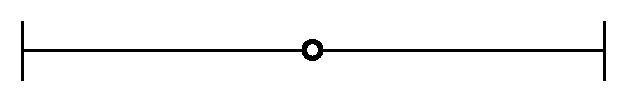
\includegraphics[width=0.45\textwidth]{quad_1d_p1}
  }
  \subfigure[$p = 3$]{
    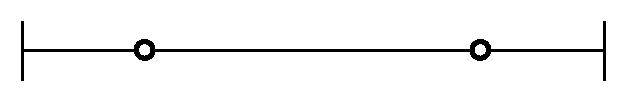
\includegraphics[width=0.45\textwidth]{quad_1d_p3}
  }
  \subfigure[$p = 5$]{
    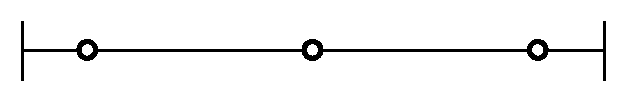
\includegraphics[width=0.45\textwidth]{quad_1d_p5}
  }
  \subfigure[$p = 7$]{
    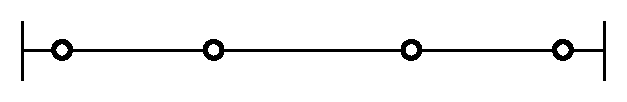
\includegraphics[width=0.45\textwidth]{quad_1d_p7}
  }
  \caption{Gauss quadrature points for $(0,1)$. \label{fig:fe_impl_gauss_points}}
\end{figure}

\begin{table}
  \centering
  \begin{tabular}{cccc}
    $p$ & $n_q$ & $\tilde \xi$ & $\tilde \rho$ \\
    \hline
    $1$ & $1$ & $0.500000000000000$ & $1.000000000000000$ \\
    \hline
    $3$ & $2$ & $0.211324865405187$ & $0.500000000000000$ \\ 
    & & $0.788675134594813$ & $0.500000000000000$ \\
    \hline
    $5$ & $3$ & $0.112701665379258$ & $0.277777777777778$ \\ 
     & & $0.500000000000000$ & $0.444444444444444$ \\ 
     & & $0.887298334620742$ & $0.277777777777778$ \\
    \hline
    $7$ & $4$ & $0.069431844202974$ & $0.173927422568727$ \\ 
    & & $0.330009478207572$ & $0.326072577431273$ \\ 
    & & $0.669990521792428$ & $0.326072577431273$ \\ 
    & & $0.930568155797026$ & $0.173927422568727$ 
  \end{tabular}
  \caption{Gauss quadrature rules for $p = 1$ to $7$ polynomials. \label{tb:fe_impl_gauss}}
  \label{tb:integ_gauss}
\end{table}

\section{Numerical quadrature in $\RR^d$}
Similar to the Gauss quadrature in $\RR^1$, there also exists efficient quadrature rules for integration of domains in $\RR^d$, $d > 1$.  If the domain is a square $[0,1]^2 \subset \RR^2$ or cube $[0,1]^3 \subset \RR^3$, then we can obtain the associated quadrature rule by the tensor-product of the one-dimensional Gauss rules; for example, for $[0,1]^2$, 
\begin{equation*}
  \int_{\tilde x_2=0}^1 \int_{\tilde x_1=0}^1 f(\tilde x_1,\tilde x_2) d\tilde x_1 d\tilde x_2
  \approx \sum_{i_2 = 0}^{n_q^{\rm 1d}} \sum_{i_1 = 0}^{n_q^{\rm 1d}} \tilde \rho_{i_2}^{\rm 1d} \tilde \rho_{i_1}^{\rm 1d} f(\tilde \xi_1^{\rm 1d}, \tilde \xi_2^{\rm 1d}).
\end{equation*}
These rules maximizes the degree of tensor-product polynomials integrated exactly for a given number of quadrature points.

For a domain in $\RR^d$, $d > 1$, that does not result from a tensor-product of a one-dimensional domain, the ``optimal'' quadrature rules are much more difficult to identify.  In fact, the optimal rules for (say) a triangle is not as universally standardized as that for a square. Table~\ref{tb:fe_impl_integ_gauss2} shows examples of efficient quadrature rule for our unit right triangle, and Figure~\ref{fig:fe_impl_integ_gauss2} visualizes the quadrature points.  Similar to the one-dimensional Gauss rule, the quadrature points are clustered towards the edge of the triangular domain.


\begin{table}
  \centering
  \begin{tabular}{ccccc}
    $p$ & $n_q$ & $\tilde \xi_1$ & $\tilde \xi_2$ & $\tilde \rho$ \\
    \hline
    $1$ & $1$ & $0.333333333333333$ & $0.333333333333333$ & $0.500000000000000$ \\
    \hline
    $2$ & $3$ & $0.166666666666667$ & $0.166666666666667$ & $0.166666666666667$ \\ 
    & & $0.666666666666667$ & $0.166666666666667$ & $0.166666666666667$ \\ 
    & & $0.166666666666667$ & $0.666666666666667$ & $0.166666666666667$ \\ 
    \hline
    $4$ & $6$ & $0.091576213509771$ & $0.091576213509771$ & $0.054975871827661$ \\ 
    & & $0.816847572980459$ & $0.091576213509771$ & $0.054975871827661$ \\ 
    & & $0.091576213509771$ & $0.816847572980459$ & $0.054975871827661$ \\ 
    & & $0.445948490915965$ & $0.445948490915965$ & $0.111690794839006$ \\
    & & $0.108103018168070$ & $0.445948490915965$ & $0.111690794839006$ \\ 
    & & $0.445948490915965$ & $0.108103018168070$ & $0.111690794839006$ \\ 
  \end{tabular}
  \caption{Gauss quadrature rules for $p = 1$ to $4$ polynomials.}
  \label{tb:fe_impl_integ_gauss2}
\end{table}

\begin{figure}
  \centering
  \subfigure[$p = 1$]{
    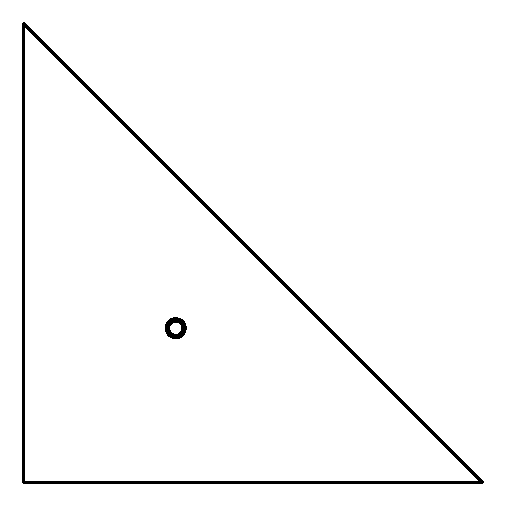
\includegraphics[width=0.23\textwidth]{quad_2d_p1}
  }
  \subfigure[$p = 2$]{
    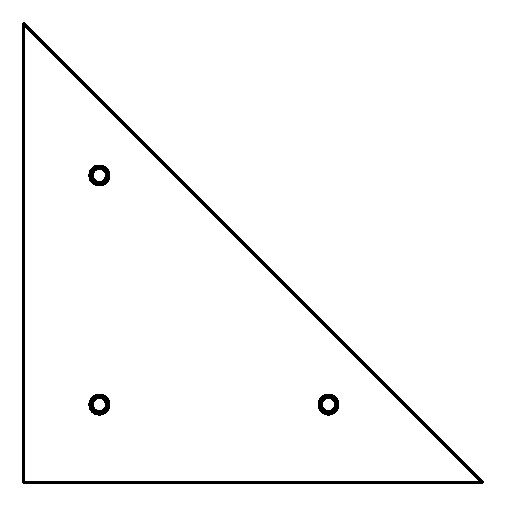
\includegraphics[width=0.23\textwidth]{quad_2d_p2}
  } 
  \subfigure[$p = 4$]{
    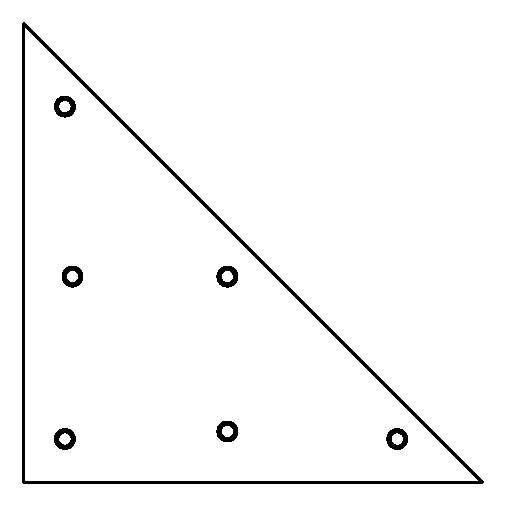
\includegraphics[width=0.23\textwidth]{quad_2d_p4}
  } 
  \subfigure[$p = 5$]{
    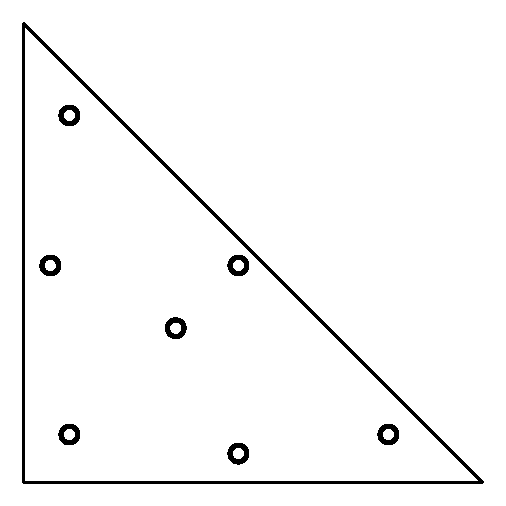
\includegraphics[width=0.23\textwidth]{quad_2d_p5}
  }
  \subfigure[$p = 6$]{
    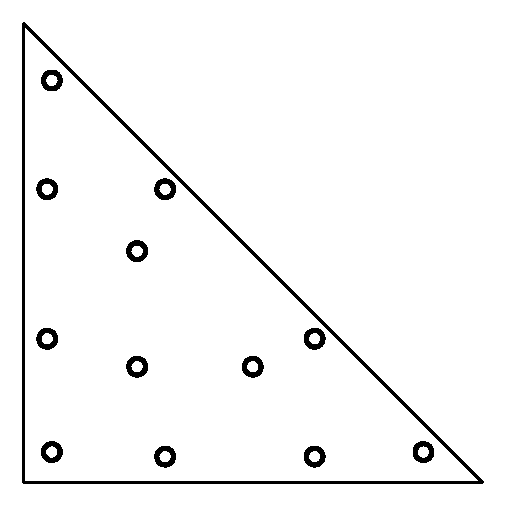
\includegraphics[width=0.23\textwidth]{quad_2d_p6}
  }
  \subfigure[$p = 7$]{
    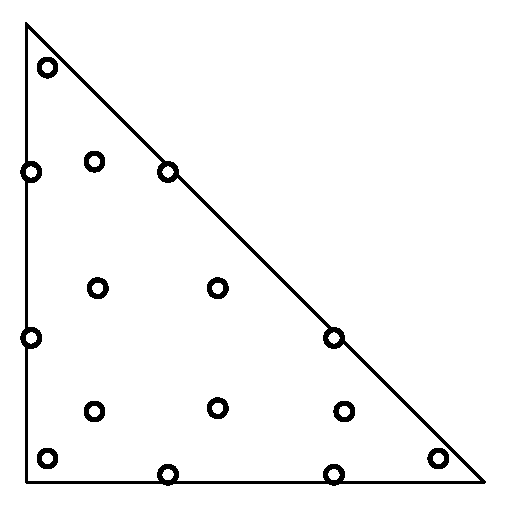
\includegraphics[width=0.23\textwidth]{quad_2d_p7}
  }
  \caption{Numerical quadrature points for the reference triangle.}
  \label{fig:fe_impl_integ_gauss2}
\end{figure}

\section{Assembly}

We have so far introduced technical ingredients required to assemble, for any $K \in \calT_h$, the local stiffness matrix $\hat A^K \in \RR^{n_s \times n_s}$ such that
\begin{equation*}
  \hat A^K_{\alpha,\beta} = a(\phi^K_\beta,\phi^K_\alpha) \quad \forall \alpha,\beta = 1,\dots,n_s,
\end{equation*}
and the local load vector $\hat f^K \in \RR^{n_s}$ such that
\begin{equation*}
  \hat f^K_\alpha = \ell(\phi^K_\alpha) \quad \forall \alpha = 1,\dots,n_s.
\end{equation*}
We now wish to assemble the local stiffness matrices and vectors construct the (global) stiffness matrix and vector.

To this end, we employ the element-to-node connectivity map,
\begin{equation*}
  \theta : \{ K_1, \dots, K_{n_e} \} \times \{ 1, \dots, n_s \} \to \{ 1,\dots,n \},
\end{equation*}
which takes in the element and local node number as the input and returns the associated global node number.  We recall that the maps is typically stored as a table of the size $n_e \times n_s$.  Then, to form the (global) stiffness matrix $\hat A_h \in \RR^{n \times n}$, we successively insert the local stiffness matrices $\hat A^K \in \RR^{n_s \times n_s}$, $K \in \calT_h$, 
\begin{equation*}
  \hat A_{h,ij} \leftarrow \hat A_{h,ij} + \hat A^K_{\alpha\beta}, \quad \forall \alpha,\beta = 1,\dots,n_s,
\end{equation*}
where $i = \theta(K,\alpha)$ and $j = \theta(K,\beta)$ are the global node indices associated with the local nodes $\alpha$ and $\beta$, respectively, of the element $K$. Similarly, to form the (global) load vector $\hat f_h \in \RR^n$, we successively insert the local load vectors $\hat f^K \in \RR^{n_s}$, $K \in \calT_h$,
\begin{equation*}
  \hat f_{h,i} \leftarrow \hat f_{h,i} + \hat f^K_{\alpha}, \quad \forall \alpha = 1,\dots,n_s,
\end{equation*}
where $i = \theta(K,\alpha)$ is the global node index associated with the local node $\alpha$ of the element $K$.


\begin{figure}
  \centering
  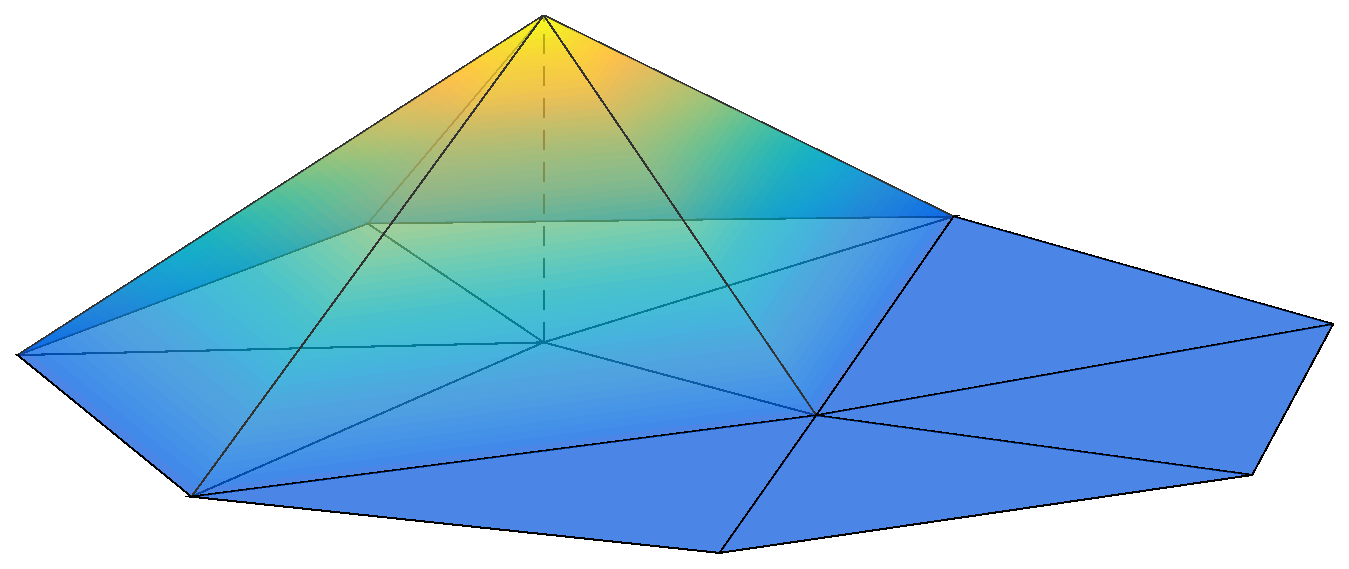
\includegraphics[width=0.48\textwidth]{shape_global_p1}
\end{figure}




%% \section{Bilinear Lagrange element on a quadrilateral}
%% We now consider arguably the simplest basis function on quadrilaterals: bilinear Lagrange basis on a reference quadrilateral.  Our reference quadrilateral is a unit square that is delineated by vertices
%% \begin{equation*}
%%   x^1 = (0,0), \quad x^2 = (1,0), \quad x^3 = (0,1), \quad \text{and} \quad x^4 = (1,1).
%% \end{equation*}
%% In two dimensions, any bilinear function can be expressed as a linear combination of monomial basis $\{ 1, x_1, x_2, x_1 x_2 \}$, which, unlike the triangular case, includes the cross term. Our interpolation points are the four vertices of the quadrilateral $\{ x^1, x^2, x^3, x^4 \}$.  Our shape functions are given by 
%% \begin{equation}
%%   \phi_i(x) = a_1^i + a_2^i x_1 + a_3^i x_2 + a_4^i x_1 x_2, \quad i = 1,\dots,4,
%%   \label{eq:fe_lin_quad_rep}
%% \end{equation}
%% where the coefficients satisfy
%% \begin{equation*}
%%   \bmat{cccc}
%%   1 & x_1^1 & x_2^1 & x_1^1 x_2^1 \\
%%   1 & x_1^2 & x_2^2 & x_1^2 x_2^2 \\
%%   1 & x_1^3 & x_2^3 & x_1^3 x_2^3 \\
%%   1 & x_1^4 & x_2^4 & x_1^4 x_2^4 \\
%%   \emat
%%   \bmat{cccc}
%%   a_1^1 & a_1^2 & a_1^3 & a_1^4 \\
%%   a_2^1 & a_2^2 & a_2^3 & a_2^4 \\
%%   a_3^1 & a_3^2 & a_3^3 & a_3^4 \\
%%   a_4^1 & a_4^2 & a_4^3 & a_4^4 \\
%%   \emat
%%   =
%%   \bmat{cccc}
%%   1 & 0 & 0 & 0 \\
%%   0 & 1 & 0 & 0 \\
%%   0 & 0 & 1 & 0 \\
%%   0 & 0 & 0 & 1
%%   \emat.
%% \end{equation*}
%% Once we find the coefficients, we can evaluate the value of the shape function at any point in the quadrilateral by evaluating~\eqref{eq:fe_lin_quad_rep}. We can also differentiate~\eqref{eq:fe_lin_quad_rep} to obtain gradient of the shape functions:
%% \begin{equation*}
%%   \pp{\phi_i}{x_1}(x) = a_2^i + a_4^ix_2
%%   \quad \text{and} \quad
%%   \pp{\phi_i}{x_2}(x) = a_3^i + a_4^ix_1, \quad i = 1,\dots,4.
%% \end{equation*}
%% Unlike the linear shape functions for triangles, the gradient of the \emph{bi}linear shape functions for quadrilateral depends on the evaluation point.


%% Formally, a finite element is defined by a triplet $(K,\calP,\Sigma)$ where
%% \begin{itemize}
%% \item[(i)] $K$ defines the domain
%% \item[(ii)] $\calP$ defines the (finite-dimensional) linear space of functions over $K$
%% \item[(iii)] $\Sigma$ defines the degrees of freedom such that a function $v \in \calP$ is uniquely determined.
%% \end{itemize}
%% For instance, for the linear Lagrange element in Section~\ref{sec:fe_lin_tri} chooses (i) the triangle as the domain $K$, (ii) space of linear functions $\PP^1(K)$ as the function space $\calP$, and (iii) the values of the function at the vertices of the triangle as the degree of freedom $\Sigma$. 

%% In general, a Lagrange basis is uniquely determined by (i) the degree of polyno




\begin{figure}
  \centering
  \subfigure[vertex shape function]{
    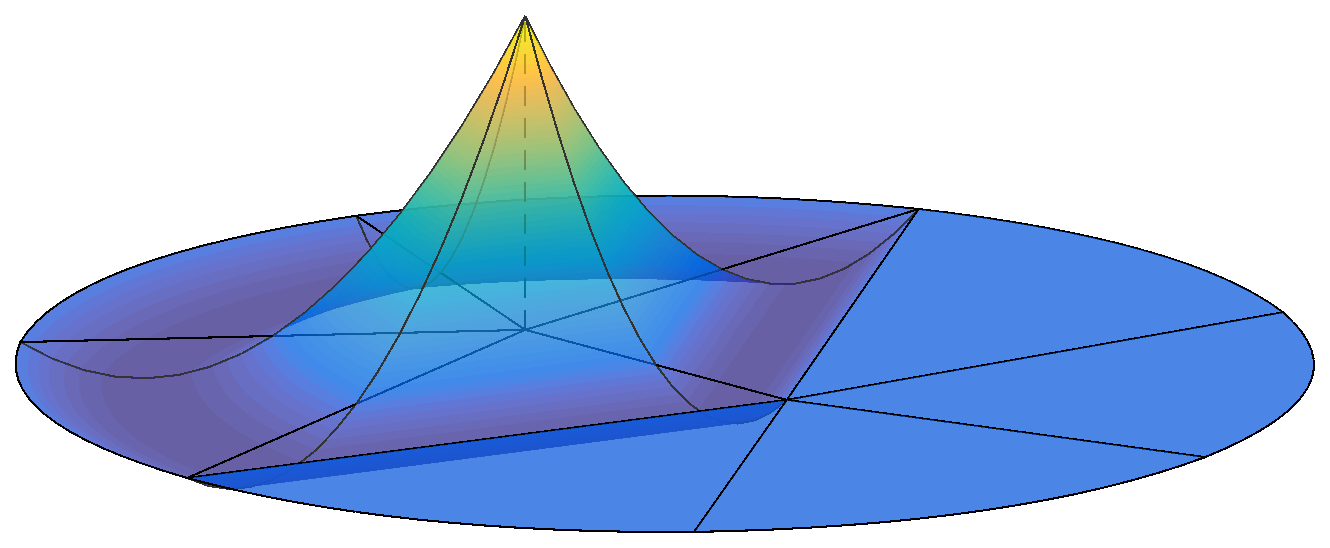
\includegraphics[width=0.48\textwidth]{shape_global_p2_1}
  }
  \subfigure[edge shape function]{
    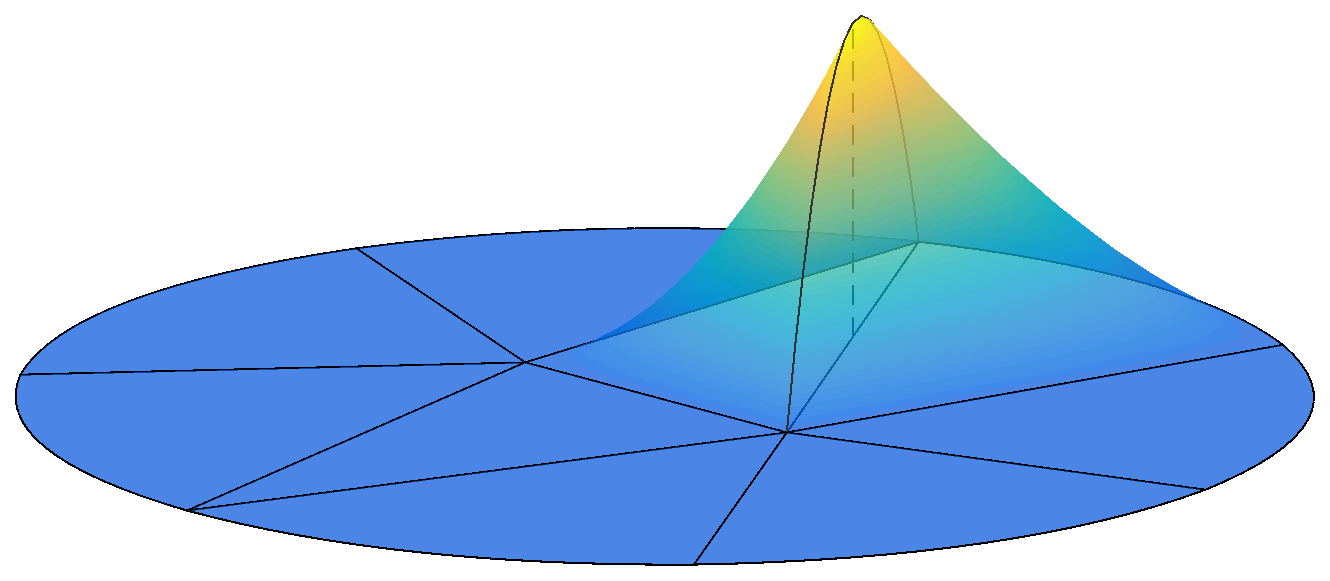
\includegraphics[width=0.48\textwidth]{shape_global_p2_2}
  }
\end{figure}


\begin{figure}
 \centering
 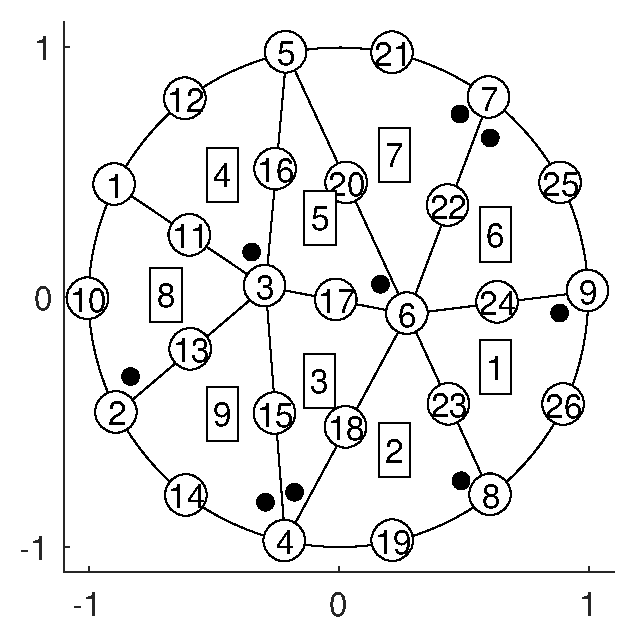
\includegraphics[width=0.4\textwidth]{fe_mesh_p2}
 \caption{$p=2$ mesh.}
 \label{fig:fe_mesh_p2}
\end{figure}
\begin{table}
  \centering
  \subfigure[coordinates]{
    \begin{tabular}{c|cc}
      node & $x_1$ & $x_2$ \\
      \hline
$1$ & $-0.89$ & $\hphantom{-}0.45$ \\ 
$2$ & $-0.89$ & $-0.46$ \\ 
$3$ & $-0.29$ & $\hphantom{-}0.04$ \\ 
$4$ & $-0.21$ & $-0.98$ \\ 
$5$ & $-0.21$ & $\hphantom{-}0.98$ \\ 
$6$ & $\hphantom{-}0.28$ & $-0.07$ \\ 
$7$ & $\hphantom{-}0.60$ & $\hphantom{-}0.80$ \\ 
$8$ & $\hphantom{-}0.61$ & $-0.79$ \\ 
$9$ & $1.00$ & $\hphantom{-}0.02$ \\ 
$10$ & $-1.00$ & $-0.01$ \\ 
$11$ & $-0.59$ & $\hphantom{-}0.25$ \\ 
$12$ & $-0.61$ & $\hphantom{-}0.79$ \\ 
$13$ & $-0.59$ & $-0.21$ \\ 
$14$ & $-0.61$ & $-0.79$ \\ 
$15$ & $-0.25$ & $-0.47$ \\ 
$16$ & $-0.25$ & $\hphantom{-}0.51$ \\ 
$17$ & $-0.01$ & $-0.01$ \\ 
$18$ & $\hphantom{-}0.03$ & $-0.52$ \\ 
$19$ & $\hphantom{-}0.22$ & $-0.98$ \\ 
$20$ & $\hphantom{-}0.03$ & $\hphantom{-}0.46$ \\ 
$21$ & $\hphantom{-}0.22$ & $\hphantom{-}0.98$ \\ 
$22$ & $\hphantom{-}0.44$ & $\hphantom{-}0.36$ \\ 
$23$ & $\hphantom{-}0.44$ & $-0.43$ \\ 
$24$ & $\hphantom{-}0.64$ & $-0.02$ \\ 
$25$ & $\hphantom{-}0.89$ & $\hphantom{-}0.46$ \\ 
$26$ & $\hphantom{-}0.90$ & $-0.43$ \\   
    \end{tabular}
  }
  \subfigure[connectivity]{
    \begin{tabular}{c|cccccc}
      element & node 1 & node 2 & node 3 & node 4 & node 5 & node 6\\
      \hline
$1$ & $9$ & $6$ & $8$ & $23$ & $26$ & $24$ \\ 
$2$ & $8$ & $6$ & $4$ & $18$ & $19$ & $23$ \\ 
$3$ & $4$ & $6$ & $3$ & $17$ & $15$ & $18$ \\ 
$4$ & $3$ & $5$ & $1$ & $12$ & $11$ & $16$ \\ 
$5$ & $6$ & $5$ & $3$ & $16$ & $17$ & $20$ \\ 
$6$ & $7$ & $6$ & $9$ & $24$ & $25$ & $22$ \\ 
$7$ & $7$ & $5$ & $6$ & $20$ & $22$ & $21$ \\ 
$8$ & $2$ & $3$ & $1$ & $11$ & $10$ & $13$ \\ 
$9$ & $4$ & $3$ & $2$ & $13$ & $14$ & $15$ \\ 
    \end{tabular}
  }
  \caption{Node coordinate and connectivity table for $p=2$ mesh shown in Figure~\ref{fig:fe_mesh_p2}}
\end{table}



%i.e., for a piecewise polynomial space $\calV_h$,
%\begin{equation*}
%  \calV_h \subset \calV \quad \Leftrightarrow \quad \calV_h \subset C^0(\overline \Omega) ,
%\end{equation*}
%where  $C^0(\overline \Omega)$ is the space of continuous functions over $\overline \Omega$.

%Given the continuity requirement, we will construct finite element spaces of the form
%\begin{equation}
%  \calV_h \equiv \{ v \in C^0(\overline \Omega) \ | v |_{K_i} \in \PP^p(K_i), \ i = 1,\dots, n_e \};
%  \label{eq:fe_space}
%\end{equation}
%we recall that $\PP^p(K_i)$ is the space of degree $p$ polynomials over $K_i$.





%% \section{Linear Lagrange element on a line segment}
%% \label{sec:fe_lin_line}
%% We first introduce arguably the simplest finite element: linear Lagrange element on a unit line segment $\tilde K$.  Our unit line segment $\tilde K \equiv (\tilde x^1, \tilde x^2)$ is delineated by two endpoints
%% \begin{equation*}
%%   \tilde x^1 = 0 \quad \text{and} \quad \tilde x^2 = 1.
%% \end{equation*}
%% For the linear polynomial space $\PP^1(\tilde K)$ and the interpolation points $\{\tilde x^1, \tilde x^2\}$, a unique set of \emph{Lagrange basis functions} (or \emph{Lagrange shape functions}) is given by
%% \begin{equation*}
%%   \tilde \phi_1(\tilde x) = 1 - \tilde x \quad \text{and} \quad \tilde \phi_2(\tilde x) = \tilde x.
%% \end{equation*}
%% Note that these basis functions satisfy the interpolation condition
%% \begin{equation*}
%%   \phi_i(\tilde x^j) = \delta_{ij}.
%% \end{equation*}
%% Here $\delta_{ij}$ is the \emph{Kronecker delta}: $\delta_{ij} = 1$ for $i = j$ and $\delta_{ij} = 0$ for $i \neq j$.

%% With these basis functions, we can describe any function $v \in \PP^1(\tilde K)$ as
%% \begin{equation*}
%%   v = \sum_{i=1}^{n_s} \tilde v_i \tilde \phi_i
%% \end{equation*}
%% for $\tilde v_i \equiv v(\tilde x^i)$, $i = 1,2$; the values of the function at the end points are the degree of freedom of the finite element.  Similarly, the derivative of the function is given by
%% \begin{equation*}
%%   \pp{v}{\tilde x} = \sum_{i=1}^{n_s} \tilde v_i \pp{\tilde \phi_i}{\tilde x},
%% \end{equation*}
%% where the direct differentiation of the basis functions yields $\pp{\tilde \phi_1}{\tilde x} = -1$ and $\pp{\tilde \phi_2}{\tilde x} = 1$.


%To see the equivalence, we observe that .  Conversely, if a polynomial space is no
%We hence choose
%\begin{equation*}
%  \calV_h \equiv \{ v \in C^0(\overline \Omega) \ | v |_{K_i} \in \PP^p(K_i), \ i = 1,\dots, n_e \};
%\end{equation*}
%



%% \section{Linear Lagrange finite element on line segments}


%% \label{sec:fe_lin_line}
%% We first introduce arguably the simplest form of finite element: linear Lagrange elements on (one-dimensional) line. In one dimension, any linear function can be expressed as a linear combination of a monomial basis
%% \begin{equation*}
%%   \{ 1, x \};
%% \end{equation*}
%% by construction, $\text{span}\{1,x\} = \PP^1(K)$. Our goal is to find the \emph{Lagrange shape functions}
%% \begin{equation*}
%%   \{ \phi_1, \phi_2 \}
%% \end{equation*}
%% that forms a basis (i.e., $\text{span}\{ \phi_1, \phi_2 \} = \PP^1(K)$) and satisfies the interpolation condition
%% \begin{equation}
%%   \phi_i(x^j) = \delta_{ij};  \label{eq:fe_interp}
%%  % \equiv
%%  % \begin{cases}
%%  %   1, \quad i = j \\
%%  %   0, \quad i \neq j
%%  % \end{cases} 
%% \end{equation}
%% here $\delta_{ij}$ is the \emph{Kronecker delta} such that $\delta_{ij} = 1$ for $i = j$ and $\delta_{ij} = 0$ for $i \neq j$.  To find the basis, we first express the shape functions in terms of the monomial basis:
%% \begin{equation}
%%   \phi_i(x) = a^i_1 + a^i_2 x \quad i = 1, 2.
%%   \label{eq:fe_lin_line_rep}
%% \end{equation}
%% We now apply the interpolation condition~\eqref{eq:fe_interp} to find the coefficients.  For instance, $\phi_1$ must satisfy
%% \begin{equation*}
%%   \bmat{cc}
%%   1 & x^1 \\
%%   1 & x^2 \\
%%   \emat
%%   \bmat{c}
%%   a_1^1 \\ a_2^1 
%%   \emat
%%   =
%%   \bmat{c}
%%   1 \\ 0 
%%   \emat
%% \end{equation*}
%% We can also pose a single matrix equation for the monomial coefficients of all three shape functions: 
%% \begin{equation*}
%%   \bmat{cc}
%%   1 & x^1 \\
%%   1 & x^2 \\
%%   \emat
%%   \bmat{cc}
%%   a_1^1 & a_1^2 \\
%%   a_2^1 & a_2^2 \\
%%   \emat
%%   =
%%   \bmat{cc}
%%   1 & 0 \\
%%   0 & 1 \\
%%   \emat.
%% \end{equation*}
%% We note that the matrix in the first matrix in the left hand side is the \emph{Vandermonde matrix} associated with our monomial basis evaluated at the vertices of the triangle.  The linear equation is well-posed as long as the interpolation points are not colinear, which is equivalent to the condition that the triangle have a finite area.

%% Once we find the coefficients of the shape functions, we can evaluate the value of the functions at any point in the triangle by evaluating~\eqref{eq:fe_lin_line_rep}. We can also differentiate~\eqref{eq:fe_lin_line_rep} to obtain the gradient of the shape functions:
%% \begin{align*}
%%   \pp{\phi_i}{x}(x) = a_2^i
%% \end{align*}
%% The derivatives are constant over the element because the shape functions are linear.


%% Using the linear Lagrange basis functions, we can now represent any function $v$ that is in $\PP^1(\tilde K)$.  Specifically, we may represent $v \in \PP^1(\tilde K)$ in terms of a coefficient vector $\hat v \in \RR^3$ as
%% \begin{equation*}
%%   v(\tilde x) = \sum_{j=1}^{3} \hat v_j  \tilde \phi_j(\tilde x) \quad \forall \tilde x \in \tilde K
%% \end{equation*}
%% for $\hat v_j \equiv v(\tilde x^j)$, $j = 1,2,3$.  We hence have a one-to-one mapping between \emph{any} element in $\PP^1(\tilde K)$ and the associated coefficient vector in $\RR^3$.  For the linear Lagrange basis functions, the coefficients $\hat v \in \RR^3$ is associated with the values of the function at the vertices of the triangle.


%% For a quadratic triangle, the mapping is quadratic and vertices and mid-edge nodes of the reference triangle are mapped to the respective vertices and mid-edge nodes of the physical triangle.

%% Formally, a finite element space is parametrized by the following three properties:
%% \begin{enumerate}
%% \item the triangulation $\calT_h$ of $\Omega$;
%% \item the type of functions that constitutes the space (e.g., piecewise linear polynomial);
%% \item the degrees of freedom used to describe functions in the space.
%% \end{enumerate}
%% The first two are apparent from the definition of the finite element space~\eqref{eq:fe_space}.  The last property determines how a function $v \in \calV_h$ is represented on a computer.  Specifically, given a $N$-dimensional function space $\calV_h$, we assign $N$ degrees of --- by choosing $N$ basis functions --- such that the a function $v \in \calV_h$ can be uniquely described by $N$ real numbers.  We will clarify this third property in Section~\ref{sec:fe_map}.
